\documentclass[11pt]{article}
\usepackage{iftex}
\usepackage[T1]{fontenc}
\usepackage{lmodern,microtype}
\usepackage[a4paper,margin=25mm,top=23mm,bottom=24mm]{geometry}
\usepackage{amsmath,amssymb,amsthm,mathtools}
\usepackage{booktabs,array,enumitem}
\usepackage{xcolor}
\usepackage[colorlinks=true,linkcolor=blue!50!black,citecolor=blue!50!black,urlcolor=blue!50!black]{hyperref}

\ifdefined\pdftrailerid\pdftrailerid{}\fi
\setlength{\emergencystretch}{1.5em}
\numberwithin{equation}{section}

\newtheorem{theorem}{Theorem}[section]
\newtheorem{proposition}[theorem]{Proposition}
\newtheorem{lemma}[theorem]{Lemma}
\newtheorem{corollary}[theorem]{Corollary}
\theoremstyle{definition}
\newtheorem{definition}[theorem]{Definition}
\theoremstyle{remark}
\newtheorem{remark}[theorem]{Remark}

\newcommand{\R}{\mathbb{R}}
\newcommand{\Q}{\mathbb{Q}}
\newcommand{\Z}{\mathbb{Z}}
\newcommand{\N}{\mathbb{N}}
\newcommand{\dd}{\,\mathrm{d}}
\newcommand{\pos}[1]{[#1]_+}
\newcommand{\Bta}{\mathrm{B}}
\DeclareMathOperator{\supp}{supp}
\DeclareMathOperator{\sgn}{sgn}
\DeclareMathOperator{\ord}{ord}
\newcommand{\Hhyp}{H_{\mathrm{hyp}}}
\newcommand{\PP}{\mathcal{P}}
% Print the companion's number on paper. The PDF checker matches #1 to its LaTeX label.
\newcommand{\othernumber}[2]{#2}
% Sibling PDF, PDF destination, source label, printed number.
\newcommand{\paperlink}[4]{\href{#1.pdf\##2}{#4}}


\ifdefined\pdfinfoomitdate\pdfinfoomitdate=1\fi
\ifdefined\pdfsuppressptexinfo\pdfsuppressptexinfo=15\fi
\newcommand{\disk}{\mathbb D}
\newcommand{\ev}{\operatorname{ev}}
\newcommand{\cL}{\mathcal L}
\newcommand{\cN}{\mathcal N}
\newcommand{\F}{\mathcal F}
\setlist{topsep=4pt}
\makeatletter\let\inputrows\@@input\makeatother

\newcommand{\splitcount}[2]{\left(#1,#2\right)_{\mathrm{terms}}}
\newcommand{\Mclr}{M_{\mathrm{clr}}}

\usepackage{tikz,placeins}
\hypersetup{pdftitle={A superquadratic lower bound for limit cycles of planar polynomial vector fields with N monomials and degree at most N-1},pdfauthor={Haibo Lu},filecolor=blue!50!black}
\title{A superquadratic lower bound for limit cycles of planar polynomial vector fields with \texorpdfstring{\(N\)}{N} monomials and degree at most \texorpdfstring{\(N-1\)}{N-1}}
\author{Haibo Lu\thanks{Shanghai Institute of Technology. ORCID: \href{https://orcid.org/0009-0000-2717-5968}{0009-0000-2717-5968}.}}
\date{November 27, 2026}
\begin{document}
\maketitle
\begin{abstract}
Let \(N\) be the number of monomials in a planar polynomial vector field, counted separately in its two components. With unrestricted degree, Gasull and Santana proved a quadratic lower bound for the number of limit cycles. We obtain a superquadratic lower bound under the additional degree cap \(N-1\). For every integer \(N\ge48\) a single field with exactly \(N\) terms, rational coefficients and coprime components has at least \(\mathcal F(N)>0\) coexisting hyperbolic limit cycles under this cap. The explicit integer \(\mathcal F(N)\) satisfies \(\mathcal F(N)\ge N^2\log_2 N-50N^2\).

The construction uses families of ovals of a separable Hamiltonian. At a saddle merger the regular coefficients before the first fractional power of the outer area integral add across the two inner families. This lets one polynomial create sign changes near several ends. Blocks of quadratic folds return a critical point to zero, raising its local order while retaining enough disjoint rows of ovals. Joint variation of the vertical potential and the perturbation on whole oval disks realizes the selected crossings in one field. With independent budgets the same argument gives \(2\Delta^2\log_2\Delta-O(\Delta^2)\) cycles at every sufficiently large exact degree \(\Delta\) using exactly \(\lceil3\Delta/2\rceil\) pure powers.
\end{abstract}
\noindent\textit{2020 Mathematics Subject Classification.} 34C07, 34C23, 37G15.\\
\textit{Keywords.} Planar polynomial vector fields, limit cycles, number of monomials, Hilbert's sixteenth problem, Abelian integrals.

\section{Introduction}\label{sec:intro}
A planar polynomial field can have few monomials of arbitrarily high degree. Conversely, a degree bound \(D\) leaves \((D+1)(D+2)\) coefficient positions in its two components. How many limit cycles can one field have when both resources are limited? We study the case of exactly \(N\) monomials and \(D\le N-1\). Thus the number of occupied positions grows linearly even though the number available grows quadratically.

In Gasull's monomial version of Hilbert's sixteenth problem the degree is free \cite[Problem~8(i)]{GasullProblems}. Buzzi, Carvalho and Gasull gave the lower bound \(N-3\) for \(N\ge4\) and a bound of order \(N\log N\) on a sequence \cite[Theorem~1.2]{BuzziCarvalhoGasull2021}. Gasull and Santana proved a quadratic lower bound for all \(N\ge9\) \cite[Theorem~1]{GasullSantana2024}. Their construction localizes successive perturbations by increasing the exponents. Its term count alone gives no linear bound on the resulting degree. We obtain an additional factor \(\log N\) while imposing the linear degree cap for every \(N\ge48\).

For \(X=(P,Q)\) let \(N(X)=|\supp P|+|\supp Q|\) after collecting ordinary monomials in fixed Cartesian coordinates and \(D(X)=\max(\deg P,\deg Q)\). An occupied monomial counts once in each component in which it occurs. Write \(\mathcal H^M(N)\) for the supremum of the isolated-cycle count at exact \(N(X)=N\) with arbitrary degree, and \(\Hhyp(m,\Delta)\) for the supremum of the hyperbolic-cycle count at exact \(N(X)=m\) and \(D(X)\le\Delta\). A hyperbolic cycle has return multiplier different from one. Our construction uses
\begin{equation}\label{eq:separable-template}
 \dot x=V'(y),\qquad \dot y=-U'(x)+\mu F(y).
\end{equation}
At \(\mu=0\) the ovals are level curves of \(U(x)+V(y)\).

\begin{theorem}[Exact term count under the cap \(N-1\)]\label{cor:linear-cap}
For each integer \(N\ge48\) there exists a field of the form \eqref{eq:separable-template} with rational coefficients, coprime components, exactly \(N\) terms and degree at most \(N-1\) having at least \(\mathcal F(N)>0\) simultaneous hyperbolic limit cycles, where \(\mathcal F(N)\) is the explicit integer defined in \eqref{eq:finite-main}. Moreover, for every \(N\ge48\),
\[
 \mathcal H^M(N)\ \ge\ \Hhyp(N,N-1)\ \ge\ \mathcal F(N)
       \ \ge\ N^2\log_2N-50N^2 .
\]
\end{theorem}

The integer \(\mathcal F(N)\) counts disjoint energy intervals on which the first-order displacement has a simple zero. At \(N=48\) it gives \(168\), whereas the simpler expression \(N^2(\log_2N-50)\) becomes positive only for \(N>2^{50}\). Under the same cap, the quadratic stationary-turn bound \(\mathcal S(N)\) of Proposition~\ref{prop:stationary-budget} exceeds \(\mathcal F(N)\) for \(48\le N<8192\), and the folded bound exceeds \(\mathcal S(N)\) for every integer \(N\ge8192\) (Section~\ref{sec:recipe}). The folded bound exceeds the elementary bound \(\mathcal E(N)\) for \(N\ge512\). Table~\ref{tab:fold} also compares it with \(\mathcal T(N)\), the count for \(\lfloor N/2\rfloor\) separate strips. With unrestricted degree, Gasull and Santana's Theorem~1 gives \(N^2/2-3N-8\) for \(N\ge9\). For these same integers the maximum within their Proposition~1 is \(4\lfloor(N-2)^2/8\rfloor\) \cite{GasullSantana2024}, \cite[\S\othernumber{sup:sources}{S1}]{LuElectronic}.

\paragraph{How the crossings coexist.}
For a regular oval enclosing the disk \(\Omega(E)\), the first-order energy displacement equals, up to orientation, \(\iint_{\Omega(E)} F'(y)\dd x\dd y\). Consider first the model \(W(X)+Z^{2\alpha}\) with \(\alpha\ge2\) even and \(W=f^2\), where \(f\) has \(q\) simple real roots and the intervening saddle heights are distinct. For example, \(W=(X^2-1)^2\) gives two inner families below energy one and a common outer family above it. In a \(q\)-well cluster there are \(q\) minima, two incoming ends at each of the \(q-1\) saddle mergers, and one outgoing end at each merger. Topology thus provides \(4q-3\) finite ends at which to study the return integral. An end contributes to the bound only when the integral changes sign on a regular energy interval.

On a component \(I\) of \(\{W<E\}\) the moment of \(Z^{2j+1}\) is \(2\int_I(E-W)^{(2j+1)/(2\alpha)}\dd X\). At a merger each regular Taylor coefficient before the first fractional power is an integral over the limiting interval, in the signed variable \(E-E_*\). The two incoming intervals meet at one point to form the outgoing interval. Canceling the incoming coefficients thus cancels the outgoing ones as well. An ordered basis of the remaining coefficients gives alternating signs on separated energy scales. The numbers of sign changes differ on minima, incoming and outgoing branches according to their fractional-term signs. Formula~\eqref{eq:Bqalpha} counts their positive parts. At \(N=48\), for example, each two-well cluster contributes ten crossings near its two minima and four near the two incoming ends. The lower bound at the outgoing end is zero. Two rows of six clusters give \(168\).

A vertical fold creates rows on which the inherited drive is even in the local coordinate. Its area integral vanishes there by reflection. Iterating the Chebyshev fold \(T_2\) alone gives local order two at zero at every depth. We tune blocks of folds to return the critical point to zero, increasing the order available for the horizontal cancellations with a summable loss of real rows. At stage \(k\), the row count grows on the scale \(2^{k+1}\) while the number of available vertical modes per row decreases on the reciprocal scale. The row count times the mode count, multiplied by the horizontal well count, contributes order \(N^2\) per stage before the losses are summed over \(\log_2 N+O(1)\) stages.

To use the coefficients of \(V\) as well as those of \(F\), one must vary the boundary of the oval disk. Lemmas~\ref{lem:whole-disk-division} and~\ref{lem:disk-core} give a regular primitive for the combined variation across the entire disk, including disks that enclose saddles. Corrections on successive rows are chosen small enough to preserve the earlier strict crossings. Rational approximation in the final physical coefficients and one common small rational \(\mu\) then give a hyperbolic cycle in each selected collar (Theorem~\ref{thm:finite-folded}).

\paragraph{Independent budgets.}
For \(h=\min(m,\Delta)\) sufficiently large and \(m\le(\Delta+1)(\Delta+2)\), the same argument gives
\[
 \Hhyp(m,\Delta)\ \ge\ h\min(2h,2m-h)\log_2h-O(h^2)
\]
with an absolute implied constant (Theorem~\ref{thm:joint-main}). The construction starts with odd \(y\)-powers in \(P\), odd \(x\)-powers in \(Q\), and positive even \(y\)-powers in \(Q\). At degree cap \(\Delta\) these three sets contain \(\lceil3\Delta/2\rceil\) positions. We call this budget \emph{saturated} for the displayed coefficient. Filling these positions gives pure powers and exact degree \(\Delta\) (Corollary~\ref{cor:degree-only}). Larger feasible exact budgets can involve mixed terms. The estimate already gives \(2\Delta^2\log_2\Delta-O(\Delta^2)\) within \(O(\Delta/\log\Delta)\) terms below saturation.

For comparison, degree alone allows constructions of order \(\Delta^2(\log\Delta)^2\). The preprints of Qin and Sun and of Lu use perturbations with mixed powers \cite{QinSun2026,LuMechanical}. Section~\ref{sec:degree-history} compares their sufficient support budgets. The lower bounds in Theorems~\ref{cor:linear-cap} and~\ref{thm:joint-main} follow from the analytic construction. The electronic supplement and source archive give finite certificates and the integer evaluations \cite{LuElectronic,LuReplay}.

\subsection{The gain from shared wells}\label{sec:related-budgets}
A simpler construction repeats one vertical potential on separate horizontal strips. At each doubling it copies existing crossings and creates new ones on outer ovals. This step is suggested by Han and Romanovski's Li\'enard construction \cite[Theorem~2.1]{HanRomanovski}. Proposition~\ref{prop:strip-product} proves the sign changes and the support count for our separate strips directly. Shared wells allow cancellation at the mergers as well. Holding their vertical potential fixed measures what the perturbation alone can achieve.

\begin{table}[!htbp]\centering\small
\caption{Coefficients in three lower bounds proved here. The diagonal is normalized by \(N^2\log_2N\) at \((m,\Delta)=(N,N-1)\), and saturation by \(\Delta^2\log_2\Delta\) at \(m=\lceil3\Delta/2\rceil\). Each coefficient is a guaranteed lower limit for hyperbolic cycles at exact term count.}\label{tab:mechanism-breakdown}
\begin{tabular}{@{}lcc@{}}\toprule
Construction & Diagonal & Saturation\\\midrule
Separate strips (Proposition~\ref{prop:strip-product}) & \(1/4\) & \(1/4\)\\
Shared wells, fixed potential (Proposition~\ref{prop:fixed-potential}) & \(1\) & \(1\)\\
Shared wells, joint variation (Theorems~\ref{cor:linear-cap} and~\ref{thm:joint-main}) & \(1\) & \(2\)\\
\bottomrule\end{tabular}
\end{table}
The diagonal coefficients for the two shared-well constructions agree. The proved losses from \(N^2\log_2N\) are \(O(N^2\log\log N)\) at fixed potential and \(O(N^2)\) under joint variation. At saturation both losses have order \(O(\Delta^2)\).
\FloatBarrier

\subsection{From simple zeros to cycles}\label{sec:regular-ovals}
A compact regular collar is a closed annulus foliated by regular ovals over a compact energy interval. We call such an energy interval a bracket when the area integral below has opposite signs at its endpoints. The following return criterion allows the same perturbation parameter on finitely many disjoint collars \cite[p.~143]{ChristopherLiTorregrosa2024}, \cite[Theorem~3, (5)]{GasullSantana2024}.
\begin{lemma}[Simultaneous hyperbolic continuation on compact regular collars]
Let $U\in\R[x]$\label{lem:hyperbolic-return} and $V,F\in\R[y]$, set $H(x,y)=U(x)+V(y)$, and suppose $\{\mathcal{C}_m\}_{m=1}^M$ is a finite family of pairwise disjoint compact annular collars in $\R^2$, each foliated by simple closed regular level curves $\gamma_{m,E}=\partial\Omega_m(E)$ of $H=E$ ($E\in[E_{-,m},E_{+,m}]$) with $|\nabla H|>0$ on $\mathcal{C}_m$. Assume that on every bracket $[E_{-,m},E_{+,m}]$, the area moment $I_m(E):=\iint_{\Omega_m(E)} F'(y)\dd x\dd y$ satisfies $I_m(E_{-,m})I_m(E_{+,m})<0$ and $|I_m'(E)|\ge c_m>0$. Then there exists $\mu_0>0$ such that for every $\mu\in(0,\mu_0)$, the system $\dot{x}=V'(y)$, $\dot{y}=-U'(x)+\mu F(y)$ possesses at least $M$ pairwise distinct, simple closed hyperbolic limit cycles, one contained in the interior of each collar $\mathcal{C}_m$.
\end{lemma}

\begin{proof}
In each collar take a transversal parametrized by energy and shorten the bracket about its simple zero, keeping opposite endpoint signs. Smooth dependence of the flow and return time gives a return map \(\Pi_{m,\mu}\) on this shorter bracket, with trajectories in the original collar. Along the flow \(\dot H=\mu F(y)\dot x\). Integration over one turn and Green's theorem give, for a fixed orientation sign \(\sigma_m\),
\[
 \frac{\Pi_{m,\mu}(E)-E}{\mu}
       \ \xrightarrow[\mu\to0]{C^1(E)}\ \oint_{\gamma_{m,E}}F(y)\dd x
       =\sigma_m I_m(E).
\]
The strict endpoint signs and derivative margin persist on all the finitely many brackets for one choice of \(\mu_0\). Each displacement then has a simple zero, hence a fixed point with positive multiplier different from one. The disjoint collars give distinct cycles.
\end{proof}

\begin{proposition}[Elementary bound]\label{thm:allocation}
For each integer \(N\ge4\) there exists a field of the form \eqref{eq:separable-template} with rational coefficients, coprime components, exactly \(N\) terms and degree at most \(N-1\) having at least
\begin{equation}\label{eq:base}
 \mathcal E(N)=\lfloor(N-2)^2/4\rfloor
\end{equation}
simultaneous hyperbolic limit cycles.
\end{proposition}
\begin{proof}
Set \(n=\lfloor(N-1)/2\rfloor,\ t=N-1-n\), so \(1+n+t=N\) and \(n(t-1)=\mathcal E(N)\).
For the elementary field take \(U=A^2T_n(x)^2,\ V=y^2\), where \(T_n(\cos\theta)=\cos n\theta\), and write \(F'(y)=\sum_{j=0}^{t-1}a_j y^{2j}\), \(F(0)=0\).
For \(c_j=\binom{2j}{j}/(4^j(j+1))\), choose
\[
 \sum_{j=0}^{t-1}c_j a_j E^j=\prod_{i=1}^{t-1}(E-i).
\]
Every \(a_j\) is a nonzero rational. On each of the \(n\) simple inverse branches of \(z=AT_n(x)\) near a zero of \(T_n\), the energy is \(z^2+y^2\), and \(A|dx/dz|\) tends smoothly to a positive constant. On compact regular energy intervals the normalized area integral therefore tends in \(C^1\), up to this constant, to \(\pi E\prod_{i=1}^{t-1}(E-i)\), by scaling the disk. All \(t-1\) zeros are simple. Choose one large integer \(A\) for all branches and one small positive rational \(\mu\) for all brackets as in Lemma~\ref{lem:hyperbolic-return}. The derivative of \(T_n^2=(1+T_{2n})/2\) uses every odd \(x\)-power through \(2n-1\). The perturbation uses the \(t\) odd \(y\)-powers through \(2t-1\) in the second component. Thus the field uses one term in the first component and \(n+t\) terms in the second. Its degree \(2\max(n,t)-1\) is at most \(N-1\), and the leading \(x\)-coefficient in the second component is a nonzero constant, giving coprimality.
\end{proof}

\begin{remark}[Filling vacant monomial positions]\label{rem:exact-fill}
Let \(X\) have degree at most \(\Delta\) and at most \(N\) terms, where \(1\le N\le(\Delta+1)(\Delta+2)\). Any prescribed finite collection of hyperbolic cycles of \(X\) persists when vacant positions of degree at most \(\Delta\) are filled with sufficiently small nonzero coefficients to give exactly \(N\) terms. The cycles persist in an open coefficient neighborhood and the two components offer \((\Delta+1)(\Delta+2)\) positions. Starting with a rational coprime pair, add a small rational multiple \(tM\) of one vacant monomial at a time. Each irreducible factor of the fixed component excludes at most one value of \(t\), since division of both \(P+t_1M\) and \(P+t_2M\) would imply division of \(P\). If the starting pair has a zero component, coprimality makes the other a nonzero constant, and the first addition may be made in the zero component.
\end{remark}

\section{Endpoint asymptotics at saddle mergers and nested horizontal potentials}\label{sec:horizontal}

Consider the model Hamiltonian $W(X)+Z^{2\alpha}$ on $\R^2$, where $\alpha\ge 2$ is an even integer and $W\in\R[X]$ is a real polynomial. At a nondegenerate maximum \(X_s\) of \(W\) the energy relative to its critical value has local form \(Z^{2\alpha}-\xi^2\), after a regular horizontal change of coordinate. The zero level has two incoming and two outgoing separatrices. The Hamiltonian linearization at \((X_s,0)\) is nonzero with square zero because \(W''(X_s)<0\) and the vertical second derivative vanishes. This is the nilpotent saddle at which the two families of ovals merge.

Away from critical values of $W$, each bounded connected component $I(E)$ of $\{X\in\R : W(X)<E\}$ defines a vertically symmetric Jordan domain $\Omega_I(E)=\{(X,Z): X\in I(E),\; |Z|<(E-W(X))^{1/(2\alpha)}\}$ bounded by a smooth regular oval. Integrating the $Z$-derivative of an odd monomial $Z^{2j+1}$ ($j\ge 0$) over $\Omega_I(E)$ yields twice the slice moment
\begin{equation}\label{eq:model-moment}
  F_{j,I}(E) := \int_{I(E)} (E-W(X))^{\gamma_j}\dd X, \qquad
  \gamma_j := \frac{2j+1}{2\alpha}, \qquad \nu_j := \gamma_j + \frac{1}{2}.
\end{equation}
Because $\alpha$ is even, $2j+1$ and $2j+1+\alpha$ are odd whereas $2\alpha$ is even; thus neither $\gamma_j$ nor $\nu_j$ is ever an integer. On any open energy interval of regular ovals, $F_{j,I}(E)$ is real-analytic in $E$.

As in the double-well example of Section~\ref{sec:intro}, each of the \(q\) minima starts a family, and each of the \(q-1\) distinct positive saddle levels ends two families and starts one enclosing family. This gives \(2q-1\) maximal annuli and \(4q-3\) finite ends. Equal heights can change the count. For \(W=T_3^2\) the three wells merge at height one, giving seven finite ends.

A regular energy bracket belongs to one specified family, and its collar is the union of the ovals in that bracket. Figure~\ref{fig:fold-geometry} illustrates the count for four wells.

\begin{figure}[htbp]
\centering
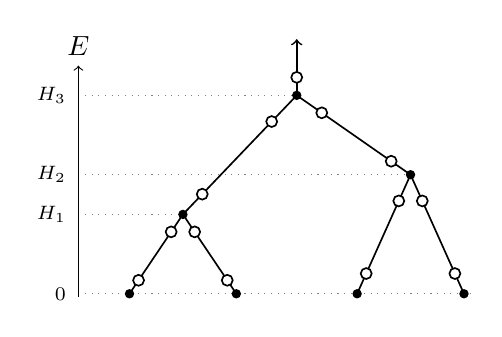
\begin{tikzpicture}[x=1.18cm,y=.84cm,
 endmark/.style={circle,draw,fill=white,inner sep=1.4pt}]
 \coordinate (a) at (0,0); \coordinate (b) at (1.15,0);
 \coordinate (c) at (2.45,0); \coordinate (d) at (3.60,0);
 \coordinate (u) at (.575,1.20); \coordinate (v) at (3.025,1.80);
 \coordinate (w) at (1.80,3.00);
 \draw[dotted,gray] (-.55,0) -- (3.70,0);
 \draw[dotted,gray] (-.55,1.20) -- (u);
 \draw[dotted,gray] (-.55,1.80) -- (v);
 \draw[dotted,gray] (-.55,3.00) -- (w);
 \foreach \start/\finish in {a/u,b/u,c/v,d/v,u/w,v/w}{
   \draw[semithick] (\start) -- node[endmark,pos=.17] {}
     node[endmark,pos=.78] {} (\finish);
 }
 \draw[semithick,->] (w) -- node[endmark,pos=.32] {} (1.80,3.85);
 \foreach \pt in {a,b,c,d,u,v,w}{\fill (\pt) circle[radius=1.7pt];}
 \draw[->] (-.55,-.05) -- (-.55,3.45) node[above] {\(E\)};
 \node[left,font=\scriptsize] at (-.58,0) {\(0\)};
 \node[left,font=\scriptsize] at (-.58,1.20) {\(H_1\)};
 \node[left,font=\scriptsize] at (-.58,1.80) {\(H_2\)};
 \node[left,font=\scriptsize] at (-.58,3.00) {\(H_3\)};
\end{tikzpicture}
\caption{Schematic of three saddle mergers for four wells at distinct heights \(H_1<H_2<H_3\). Edges represent maximal period annuli. Hollow circles mark the two finite ends of each bounded edge and the single finite end of the outer edge, thirteen in all. The lower bound for crossings near each marked end depends on its type and on the available modes in \eqref{eq:Bqalpha}.}
\label{fig:fold-geometry}
\end{figure}


At a merger the outer limiting interval is the union of the two inner intervals up to the saddle point. At a saddle height \(H_*\), each coefficient of \((E-H_*)^\ell\) for an integer \(0\le\ell<\nu_j\) in the slice moment \(F_{j,I}\) is a convergent integral over that interval. The two incoming sets of cancellations thus suffice for all three one-sided families. For nilpotent double loops, Yang, Yu and Han obtain a constant-term addition law \cite[(3.17)]{YangYuHan2019} and higher coefficients for centrally symmetric cuspidal loops under recursive analytic hypotheses \cite[Theorem~3.1]{YangYuHan2021}. For a hyperbolic saddle Xu, Yang and Han record the regular addition law \cite[(1.5)--(1.6)]{XuYangHan2024}, citing \cite{HanYangLi2023}. Here the slice integral gives every coefficient preceding its first fractional power, together with the one-sided signs needed to count crossings.

\FloatBarrier
\begin{lemma}[Local expansions and intrinsic signs at extrema]\label{lem:saddle-singular}
Fix $j\ge 0$, write $\gamma=\gamma_j$, $\nu=\nu_j$, $k_j=\lfloor\nu\rfloor$, and let $v>0$ denote the energy distance $\lvert E-E_*\rvert$ to a Morse critical value $E_*$ of $W$.
\begin{enumerate}[label=(\alph*),nosep]
  \item At a nondegenerate local minimum of height $E_*=0$, $F_{j,I}(v)=c_0 v^\nu(1+O(v))$ as $v\downarrow 0$ with $c_0>0$.
  \item Suppose a nondegenerate maximum of height $E_*=H_*$ joins two bounded sublevel intervals into one and the two outer turning points at that height are simple. On each of the two incoming branches ($E=H_*-v$) and on the outgoing branch ($E=H_*+v$), one has as $v\downarrow 0$
  \begin{equation}\label{eq:local-saddle-jet}
    F_{j,I}(H_*\pm v) = \sum_{\ell=0}^{k_j} A_{\ell,I} (\pm v)^\ell + C_I v^\nu + o(v^\nu),
  \end{equation}
  where $\sgn C_I = (-1)^{k_j+1}$ on each incoming branch and $\sgn C_I = \sgn(\gamma-k_j)$ on the outgoing branch. Moreover, for every $0\le\ell\le k_j$, the outgoing signed-energy Taylor coefficient $A_{\ell,\mathrm{out}}$ equals the sum $A_{\ell,\mathrm{in},-}+A_{\ell,\mathrm{in},+}$ of the two incoming signed-energy Taylor coefficients.
\end{enumerate}
\end{lemma}

\begin{proof}
At a nondegenerate minimum, choose a local analytic Morse coordinate $w$ with $W(X)=w^2$ and $\dd X/\dd w = A_0(w)>0$. Rescaling $w=\sqrt{v}\,u$ gives $F_{j,I}(v)=v^\nu\int_{-1}^1 (1-u^2)^\gamma A_0(\sqrt{v}\,u)\dd u = A_0(0)\Bta(\tfrac{1}{2},\gamma+1)v^\nu(1+O(v))$, proving~(a).

Near a nondegenerate maximum $X_*$ with $W(X_*)=H_*$, choose an orientation-preserving analytic coordinate $w$ on $[-c,c]$ ($c>0$) such that $W(X)=H_*-w^2$ and $\dd X/\dd w = A(w)>0$. Apart from the saddle and neighborhoods of the simple outer turning points, $H_*-W(X)$ is bounded below by a positive constant on the remaining compact intervals. Taking $W$ itself as local coordinate near a simple outer turning point $X_{\mathrm{turn}}(E)$ shows that $\int (E-W)^\gamma (\dd X/\dd W)\dd W$ extends smoothly in $E$ across $E=H_*$. Thus all non-smoothness at $E=H_*$ comes from the local integral over $w\in[-c,c]$.

On the right incoming branch ($E=H_*-v$, $w\in[\sqrt{v},c]$; the left branch $w\in[-c,-\sqrt{v}]$ is identical with $A(-w)$), the local integral is $\int_{\sqrt{v}}^c (w^2-v)^\gamma A(w)\dd w$. Substituting $t=w^2-v$ gives
\[
  \frac{1}{2}\int_0^{c^2-v} t^\gamma (t+v)^{-1/2} A\bigl(\sqrt{t+v}\bigr)\dd t.
\]
Expand $A(\pm\sqrt{s})=A(0)\pm s^{1/2}B_1(s)+s B_2(s)$ with $B_1,B_2$ analytic near $s=0$. Differentiate $k_j+1$ times with respect to $v$:
\begin{itemize}[nosep]
  \item Boundary terms at the upper limit $c^2-v$ are smooth and $O(1)$ as $v\downarrow 0$.
  \item For the odd-coordinate piece $\pm(t+v)^{1/2}B_1(t+v)$, the singular factor $(t+v)^{-1/2}$ cancels $(t+v)^{1/2}$ identically, leaving the analytic function $\pm B_1(t+v)$ whose $(k_j+1)$-st $v$-derivative is bounded on $[0,c^2-v]$ and contributes $O(1)$.
  \item The even remainder $(t+v)^{-1/2}\cdot(t+v)B_2(t+v)=(t+v)^{1/2}B_2(t+v)$ has $(k_j+1)$-st $v$-derivative $O((t+v)^{-k_j-1/2})$, whose integral against $t^\gamma$ is $O(1)$ (for $k_j=0$ it integrates directly to $O(1)$, and for $k_j\ge 1$ scaling $t=vz$ near $0$ gives $O(v^{\nu-k_j})+O(1)=O(1)$ since $\nu>k_j$).
  \item The principal $A(0)$ piece gives $\frac{1}{2}A(0)(-1)^{k_j+1}(\tfrac{1}{2})_{\overline{k_j+1}}\int_0^{c^2-v} t^\gamma(t+v)^{-k_j-3/2}\dd t$. Here \((a)_{\overline m}=\prod_{j=0}^{m-1}(a+j)\). Scaling $t=vz$ yields
  \[
    \frac{1}{2}A(0)(-1)^{k_j+1}\bigl(\tfrac{1}{2}\bigr)_{\overline{k_j+1}}\Bta\bigl(\gamma+1,\,k_j+\tfrac{1}{2}-\gamma\bigr)v^{\nu-k_j-1} + O(1),
  \]
  where the Beta integral converges since $\gamma>-1$ and $k_j+\frac{1}{2}-\gamma=k_j+1-\nu>0$.
\end{itemize}
Since $\nu-k_j-1\in(-1,0)$, integrating $k_j+1$ times from $0$ to $v$ divides by $(\nu)_{\underline{k_j+1}}=\nu(\nu-1)\cdots(\nu-k_j)>0$ (every factor is strictly positive because $k_j<\nu<k_j+1$) and produces~\eqref{eq:local-saddle-jet} on each incoming side with $\sgn C_{\mathrm{in}}=(-1)^{k_j+1}$.

On the outgoing branch ($E=H_*+v$), we integrate $(w^2+v)^\gamma A(w)$ over $[-c,c]$. The odd part of $A(w)$ cancels, leaving $\int_{-c}^c (w^2+v)^\gamma(A(0)+w^2 B_2(w^2))\dd w$. Differentiating $k_j+1$ times with respect to $v$ under the integral gives $(\gamma)_{\underline{k_j+1}}\int_{-c}^c (w^2+v)^{\gamma-k_j-1}(A(0)+O(w^2))\dd w$. Rescaling $w=\sqrt{v}\,z$, the $O(w^2)$ error is $O(1+v^{\nu-k_j})=O(1)$, while the $A(0)$ term gives $A(0)(\gamma)_{\underline{k_j+1}}\Bta(\tfrac{1}{2},k_j+\tfrac{1}{2}-\gamma)v^{\nu-k_j-1}+O(1)$ (convergent since $k_j+\frac{1}{2}-\gamma>0$). In $(\gamma)_{\underline{k_j+1}}=\gamma(\gamma-1)\cdots(\gamma-k_j)$, the first $k_j$ factors satisfy $\gamma-(k_j-1)=\nu-k_j+\frac{1}{2}>\frac{1}{2}>0$, so $\sgn(\gamma)_{\underline{k_j+1}}=\sgn(\gamma-k_j)$. Integrating $k_j+1$ times divides by $(\nu)_{\underline{k_j+1}}>0$, establishing $\sgn C_{\mathrm{out}}=\sgn(\gamma-k_j)$.

It remains to identify the regular coefficients on the three sides. Write \(\beta=\gamma-\ell\) for \(0\le\ell\le k_j\), so \(\beta>-1/2\). At a regular energy the first \(\ell\) signed-energy derivatives have integrands \((\gamma)_{\underline{\ell}}(E-W)^\beta\). Indeed, before each differentiation the power at a simple turning point is positive, so its boundary term vanishes, and the resulting power is locally integrable. To pass to \(E=H_*\), fix an interior cutoff \(X_0\) near each simple outer turning point on a monotone branch of \(W\). In \(u=E-W(X)\) that endpoint piece, omitting the constant factor, is
\[
  \int_0^{E-W(X_0)} u^\beta
     \left|(W^{-1})'(E-u)\right|\,\mathrm du .
\]
The inverse derivative is smooth and bounded on the chosen branch. The upper limit tends to a positive number, and \(\beta>-1\) gives convergence at \(u=0\). On the compact parts away from turning points and the saddle the integrands converge uniformly.

In the saddle chart alone, split at \(|w|=2\sqrt v\). On \(2\sqrt v\le |w|\le c\), the factors \(w^2\pm v\) are comparable to \(w^2\), so \(C|w|^{2\beta}\) is an integrable majorant. In the inner part put \(w=\sqrt v\,z\). Its absolute contribution is \(O(v^{\beta+1/2})=O(v^{\nu-\ell})\). The rescaled integral contains \((z^2+1)^\beta\) on \(|z|\le2\) above the saddle, or \((z^2-1)^\beta\) on \(1\le|z|\le2\) below, both integrable. Thus on each side
\[
 A_{\ell,I}=\frac{(\gamma)_{\underline{\ell}}}{\ell!}
      \int_{I(H_*)}(H_*-W(X))^{\gamma-\ell}\,\mathrm dX .
\]
The limiting outgoing interval is the union of the two incoming intervals up to the saddle point. Additivity of the displayed integrals gives the asserted identity for the signed-energy Taylor coefficients.
\end{proof}

Write $\pos{t}=\max(t,0)$. For integers $q\ge 2$, $\alpha\ge 2$ even, and $L\ge 1$, set $B_{q,\alpha}(0):=0$ and
\begin{equation}\label{eq:Bqalpha}
  \begin{gathered}
    b := \left\lfloor\frac{L-1+\alpha/2}{\alpha}\right\rfloor, \qquad
    c := \left\lfloor\frac{2(L-1)}{\alpha}\right\rfloor, \qquad
    J := L - 2(q-1)(b+1) - 1, \\
    B_{q,\alpha}(L) := q\pos{J} + 2(q-1)\pos{J-b} + (q-1)\pos{J-c}.
  \end{gathered}
\end{equation}

\begin{lemma}[Simultaneous endpoint brackets on a $q$-well cluster]\label{lem:endpoint-cluster}
Let $f\in\R[X]$ be a polynomial of degree $q\ge 2$ with $q$ simple real roots and $q-1$ critical points at which $f^2$ takes pairwise distinct positive values, and put $W=f^2$. For every even $\alpha\ge 2$ and every integer $L\ge 1$, there exists an odd rational polynomial $S\in\Q[Z]$ of degree at most $2L-1$ whose integrated derivative $\iint_{\Omega_I(E)} S'(Z)\dd X\dd Z$ has at least $\pos{J}$ regular energy brackets near each minimum, $\pos{J-b}$ on each incoming saddle branch and $\pos{J-c}$ on each outgoing branch, for a total of at least $B_{q,\alpha}(L)$. Their compact annular collars are pairwise disjoint in the $(X,Z)$-plane. On each bracket the moment has opposite endpoint signs and its energy derivative is bounded strictly away from zero.
\end{lemma}

\begin{proof}
If $J\le 0$ then $B_{q,\alpha}(L)=0$ and any rational $S$ suffices; assume $J\ge 1$. Consider $S(Z)=\sum_{j=0}^{L-1} a_j Z^{2j+1}$ with coefficient vector $a=(a_0,\dots,a_{L-1})\in\R^L$. Note that $\max_{0\le j<L}\lfloor\nu_j\rfloor=\lfloor\frac{L-1}{\alpha}+\frac{1}{2}\rfloor=b$. At each of the $q-1$ distinct saddle heights $H_*$ and on each of its two incoming branches, impose the $b+1$ homogeneous linear equations $\sum_{j:\,\ell<\nu_j} A_{\ell,I}^{(j)} a_j = 0$ ($0\le\ell\le b$), where $A_{\ell,I}^{(j)}$ is the signed-energy Taylor coefficient of $F_{j,I}$ from Lemma~\ref{lem:saddle-singular}(b). There are $2(q-1)(b+1)$ homogeneous linear equations on $\R^L$, so their joint real kernel $\mathcal N$ has dimension $n_0\ge L-2(q-1)(b+1)=J+1\ge 2$ without any independence assumption on the rows. By Lemma~\ref{lem:saddle-singular}(b), every $a\in\mathcal N$ also satisfies $\sum_{j:\,\ell<\nu_j} A_{\ell,\mathrm{out}}^{(j)} a_j=0$ ($0\le\ell\le b$) at every saddle.

Choose a row-echelon basis $v^{(0)},\dots,v^{(n_0-1)}$ of $\mathcal N$ ordered by strictly increasing first nonzero column indices $0\le p_0<p_1<\cdots<p_{n_0-1}\le L-1$, normalized to have $v^{(i)}_{p_i}=1$ and $v^{(i)}_j=0$ for $j<p_i$. Fix $i\in\{0,\dots,n_0-1\}$. Because every nonzero entry $v^{(i)}_j$ has $j\ge p_i$, for each integer $\ell<\nu_{p_i}$ we also have $\ell<\nu_j$, so all columns occurring in $v^{(i)}$ participate in row $\ell$ and cancel the $\ell$-th Taylor term exactly. Every uncanceled integer Taylor term has order $\ell>\nu_{p_i}$, and columns $j>p_i$ have fractional order $\nu_j>\nu_{p_i}$. Therefore, on every incoming and outgoing saddle branch $I$, the moment of $v^{(i)}$ has leading asymptotic $2 C_I^{(p_i)} v^{\nu_{p_i}}(1+o(1))$ as $v=|E-H_*|\downarrow 0$, with the intrinsic sign of column $p_i$ from Lemma~\ref{lem:saddle-singular}(b), while at each of the $q$ minima ($E=v\downarrow 0$) it has positive leading term $2c_{0,I}^{(p_i)} v^{\nu_{p_i}}(1+o(1))$.

To separate the leading orders of the saddle moments, fix an integer $A_0>L$, let $\rho\in(0,1)$, and form $a(\rho)=\sum_{i=0}^{n_0-1}(-1)^i\rho^{(A_0-p_i)^2} v^{(i)}$. Evaluate at the $n_0$ energy offsets $v_m=\rho^{2\alpha(A_0-p_m)}$ ($0\le m<n_0$). Since $\nu_{p_i}=\nu_0+p_i/\alpha$, the leading term of $v^{(i)}$ at $v_m$ has magnitude proportional to
\[
  \rho^{(A_0-p_i)^2 + 2\alpha(A_0-p_m)(\nu_0+p_i/\alpha)}
  = \rho^{2\alpha(A_0-p_m)\nu_0 + A_0^2 - p_m^2 + (p_i-p_m)^2}.
\]
Every $i\ne m$ carries an extra positive exponent $(p_i-p_m)^2\ge 1$ in $\rho$, and the remainder of the dominant column is \(o(1)\) relative to its leading term as \(v_m\downarrow0\). Hence for a single sufficiently small $\rho\in(0,1)$, the moment at offset $v_m$ from each of the $4q-3$ finite ends has sign $(-1)^m$ times the intrinsic sign of column $p_m$. Along the full list $j=0,\dots,L-1$:
\begin{itemize}[nosep]
  \item at each minimum the intrinsic sign is $+1$ ($0$ switches), giving $n_0-1\ge J$ sign changes;
  \item on each incoming branch $\lfloor\nu_j\rfloor=\lfloor(j+\alpha/2)/\alpha\rfloor$ increases from $0$ to $b$ in unit steps ($b$ switches), so its restriction to $p_0<\cdots<p_{n_0-1}$ switches at most $b$ times, leaving at least $\pos{n_0-1-b}\ge\pos{J-b}$ sign changes;
  \item on each outgoing branch $\sgn(\gamma_j-\lfloor\nu_j\rfloor)$ is $+1$ for $0\le(j\bmod\alpha)<\alpha/2$ and $-1$ for $\alpha/2\le(j\bmod\alpha)<\alpha$, switching $c=\lfloor 2(L-1)/\alpha\rfloor$ times along $0,\dots,L-1$, hence leaving at least $\pos{J-c}$ sign changes.
\end{itemize}
Choose \(\rho\) small enough that the energy intervals for different critical heights are disjoint. This also separates the intervals drawn from the two ends of any one bounded annulus. Near height zero the collars lie in disjoint wells. At one saddle the two incoming families lie in disjoint components below the critical energy, and the outgoing family lies above it. Summing over $q$ minima, $2(q-1)$ incoming branches, and $q-1$ outgoing branches gives at least $B_{q,\alpha}(L)$ strict sign-changing brackets.

Approximate $a(\rho)$ by a rational vector preserving the strict signs at all the chosen energies. Adding $\tau Z$ changes the moment by $2\tau F_{0,I}(E)$. On every regular oval, $F_{0,I}(E)>0$, and on each compact sign-changing bracket the ratio $-M_I(E)/(2F_{0,I}(E))$ is real-analytic and nonconstant (by its opposite endpoint signs), so its derivative vanishes at only finitely many energies there. Choosing a single small rational $\tau$ avoiding this finite set of critical values across all brackets while keeping the endpoint signs strict produces a simple zero in the interior of every bracket. Choose a compact subinterval strictly inside each crossing interval about one such zero. Its energy derivative is bounded away from zero. The subintervals separate even consecutive crossings with a common sample endpoint. Enclosed disks may nest, but their selected collars are disjoint. Lemma~\ref{lem:hyperbolic-return} then counts distinct cycles for one perturbation parameter.
\end{proof}
The vertical rows will use clusters of different sizes. Nesting the smaller groups of wells inside larger ones lets all these rows use the same horizontal polynomial and hence the same powers of \(x\).
The inner tilts can break reflection symmetry. An even-degree outer Chebyshev polynomial restores an even potential in the physical variable. Its paired simple roots then give every odd power in the derivative. In the case \(L=0\) below we use \(\deg 0=-\infty\), so a negative degree bound permits only the zero polynomial.
\begin{lemma}[Gluing dyadic horizontal group sizes in one potential]\label{lem:horizontal-glue}
Let $q_{\max}\ge 2$ be a power of two and $s\ge 2$ be an even integer. Given any finite collection of triples $(q,\alpha,L)$ with $q\in\{2,4,\dots,q_{\max}\}$ dyadic, $\alpha\ge 2$ even, and $L\ge 0$, there exists one even rational polynomial $W\in\Q[x]$ of degree $2X_*$ ($X_*:=q_{\max} s$) such that:
\begin{enumerate}[label=(\alph*),nosep]
  \item for each triple $(q,\alpha,L)$ in the collection, a rational odd polynomial $S\in\Q[Z]$ of degree at most $2L-1$ produces at least $(X_*/q)B_{q,\alpha}(L)$ simple-zero brackets for $\iint_{\Omega(E)}S'(Z)\dd x\dd Z$ on regular oval branches of $W(x)+Z^{2\alpha}$. The compact annular collars for this triple are pairwise disjoint in the $(x,Z)$-plane;
  \item the derivative $W'(x)$ contains with nonzero coefficients precisely the $X_*$ odd powers $x,x^3,\dots,x^{2X_*-1}$.
\end{enumerate}
\end{lemma}

\begin{proof}
Begin at $q_1=2$ with $f_2(X)=X^2-1$, which has two simple roots $\pm 1$ and one critical point $0$ with $f_2(0)^2=1>0$; choose the rational primitives and compact simple-zero brackets of Lemma~\ref{lem:endpoint-cluster} for all triples in the collection having $q=2$. Inductively, suppose $f_q\in\Q[X]$ ($2\le q<q_{\max}$ dyadic) has $q$ simple real roots and $q-1$ simple real critical points with pairwise distinct nonzero values of $f_q^2$, together with fixed compact simple-zero brackets for all assigned triples up to size $q$. Set $g(X):=f_q(T_2(X)/\epsilon_q)$ with $T_2(X)=2X^2-1$ and rational $\epsilon_q>0$ small. Near each simple root $\pm 1/\sqrt{2}$ of $T_2$, the coordinate $u=T_2(X)/\epsilon_q$ has normalized inverse Jacobian $\epsilon_q^{-1}|\dd X/\dd u|\to 2^{-3/2}$ in $C^2$ on every fixed compact $u$-interval as $\epsilon_q\downarrow 0$, while the new central barrier $g(0)^2=f_q(-1/\epsilon_q)^2\to+\infty$ lies strictly above all compact energy brackets already chosen on $f_q^2$. Thus for small rational $\epsilon_q>0$, $g$ has $2q$ simple real roots, $2q-1$ interlacing simple real critical points with $g(c)\ne 0$, and two disjoint copies of every previously selected compact simple-zero bracket.

Now set $f_{2q}(X):=g(X)+\delta_q(a_q+b_q X)$ with $(a_q,b_q)\in\Q^2$ and rational $\delta_q>0$ small. At each continued critical point $c(\delta_q)$ of $f_{2q}$, differentiating $f_{2q}(c(\delta_q))^2$ at $\delta_q=0$ gives $2g(c(0))(a_q+b_q c(0))$ because $g'(c(0))=0$. Since $g(c(0))\ne 0$, for any two distinct critical points $c_1\ne c_2$ with $g(c_1)^2=g(c_2)^2$, equality of first derivatives $\pm(a_q+b_q c_1)=a_q+b_q c_2$ defines a proper line in $\R^2$ (for $+$, $b_q(c_1-c_2)=0\implies b_q=0$; for $-$, $2a_q+b_q(c_1+c_2)=0$, nontrivial even if $c_1=-c_2\ne 0$). Choosing $(a_q,b_q)\in\Q^2$ outside these finitely many lines and taking rational $\delta_q>0$ sufficiently small splits all $2q-1$ squared critical values of $f_{2q}$ while preserving the $2q$ simple real roots and all inherited simple-zero brackets by $C^1(E)$ openness. Now apply Lemma~\ref{lem:endpoint-cluster} to $f_{2q}^2$ for all triples assigned to $2q$. Repeating up to $q_{\max}$ gives $f_{q_{\max}}\in\Q[X]$, with $q_{\max}/q$ copies of each bracket chosen at size $q$.

Finally, define $W(x):=f_{q_{\max}}(T_s(x)/\epsilon)^2$ for a sufficiently small rational $\epsilon>0$. Near each of the $s$ simple real zeros $x_m=\cos(\frac{(2m-1)\pi}{2s})$ of $T_s$, $u=T_s(x)/\epsilon$ has $\epsilon^{-1}|\dd x/\dd u|\to |T_s'(x_m)|^{-1}>0$ in $C^2$ on compact sets, producing $s$ disjoint copies of the entire $q_{\max}$-well hierarchy and hence $(s q_{\max}/q)B_{q,\alpha}(L)=(X_*/q)B_{q,\alpha}(L)$ simple-zero brackets for every triple; this proves~(a).

For~(b), although $f_{q_{\max}}(X)$ need not be even in $X$ after the linear tilts, $s$ is \emph{even}, so $T_s(-x)=T_s(x)$ and hence $\phi(x):=f_{q_{\max}}(T_s(x)/\epsilon)$ is an \emph{even} polynomial in $x$ of degree $X_*=q_{\max} s$. For small $\epsilon>0$, each of the $q_{\max}$ simple real roots $r_l$ of $f_{q_{\max}}$ satisfies $|\epsilon r_l|<1$ and therefore pulls back under $T_s$ to $s$ distinct simple real roots in $(-1,1)$ (none equal to $0$ since $T_s(0)=(-1)^{s/2}=\pm 1\ne\epsilon r_l$). Thus $\phi$ has $X_*$ simple real roots, Rolle's theorem supplies $X_*-1$ interlacing simple real roots of $\phi'$, and $W'(x)=2\phi(x)\phi'(x)$ is an odd polynomial of degree $2X_*-1$ with $2X_*-1$ distinct simple real roots. One root is $0$ and the remaining $2X_*-2$ come in opposite pairs $\pm\xi_1,\dots,\pm\xi_{X_*-1}$ ($\xi_l>0$ distinct). Consequently
\[
  W'(x) = c_* x \prod_{l=1}^{X_*-1} (x^2-\xi_l^2), \qquad c_*\in\Q\setminus\{0\}.
\]
Every coefficient of $\prod_{l=1}^{X_*-1}(x^2-\xi_l^2)$ in $x^2$ is $(-1)^{X_*-1-k} e_{X_*-1-k}(\xi_1^2,\dots,\xi_{X_*-1}^2)\ne 0$, so $W'(x)$ has nonzero coefficients on precisely $x,x^3,\dots,x^{2X_*-1}$.
\end{proof}

\section{Recurrent quadratic folds and division on an oval disk}\label{sec:folds}

\subsection{Recurrent critical-returning quadratic folds}

A cluster of \(q\) wells supplies \(4q-3\) one-sided finite ends for the moment estimates. At its \(q-1\) saddles Lemma~\ref{lem:endpoint-cluster} imposes \(2(q-1)(b+1)\) linear conditions on \(L\) coefficients, with \(b=\lfloor(L-1)/\alpha+1/2\rfloor\). To retain free coefficients in this estimate as the clusters grow, we increase the vertical exponent \(2\alpha\). In the diagonal construction \(\alpha=2e\), where \(e\) is the local order of the remaining fold at zero. Ordinary iteration of \(T_2(z)=2z^2-1\) sends \(0\) to \(-1\), then to the fixed point \(1\), and has local order \(e=2\) at zero at every positive depth. At \(\alpha=4\) one has \(4(b+1)\ge L\). For \(q\ge3\) the count \eqref{eq:Bqalpha} then gives zero, independently of the actual rank of the conditions.

We group the quadratic maps into blocks that return zero to zero with local order two, so the local orders of complete blocks multiply under composition. A block of length \(\ell\) retains at least \(2^\ell-4\) simple real inverse branches over each interior value. Increasing the block lengths lets the clusters grow while keeping the loss of rows and the cost of cancellation at each saddle within the bounds used in Section~\ref{sec:sum}.

Let $T_d(\cos\theta)=\cos(d\theta)$. For each integer $\ell\ge 4$, define a tuned block of $\ell$ quadratic maps by composing $c_\ell T_2$ first and then $\ell-1$ copies of $T_2$:
\begin{equation}\label{eq:Pl-block}
  b_\ell^* := 2^{\ell-1}, \qquad c_\ell := \cos\left(\frac{\pi}{2^{\ell}}\right), \qquad
  P_\ell(z) := T_{b_\ell^*}\bigl(c_\ell T_2(z)\bigr), \qquad T_2(z)=2z^2-1.
\end{equation}
Because $b_\ell^*=2^{\ell-1}\ge 8$ is even, $T_{b_\ell^*}$ is even and $T_{b_\ell^*}(\pm c_\ell)=\cos(\pi/2)=0$ with $T_{b_\ell^*}'(\pm c_\ell)\ne 0$. Hence $P_\ell(0)=T_{b_\ell^*}(-c_\ell)=0$ with $\ord_0 P_\ell=2$ (since $T_2(z)=-1+2z^2$), while $P_\ell(\pm 1)=T_{b_\ell^*}(c_\ell)=0$ with $P_\ell'(\pm 1)\ne 0$ (local degree $1$). For $\ell=4$, Figure~\ref{fig:fold-block} illustrates the critical return at zero and the twelve simple interior preimages of $1/2$.

\begin{figure}[htbp]
\centering
\(\displaystyle
 0 \xrightarrow[\text{order }2]{\,c_4T_2\,} -c_4
   \xrightarrow[\text{order }1]{\,T_8\,} 0,
 \qquad
 P_4=T_8\circ(c_4T_2),\quad c_4=\cos(\pi/16)
\)\par\medskip
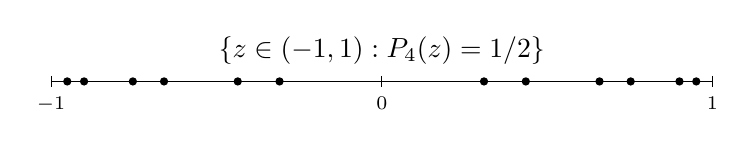
\begin{tikzpicture}[x=4.2cm,y=1cm]
 \draw[semithick] (-1,0)--(1,0);
 \foreach \x in {-1,0,1}{
    \draw (\x,.07)--(\x,-.07) node[below,font=\scriptsize] {\(\x\)};
 }
 \foreach \a in {5,7,11,13,17,19}{
   \pgfmathsetmacro{\xx}{sqrt((1+cos(7.5*\a)/cos(11.25))/2)}
   \fill (\xx,0) circle[radius=1.5pt];
   \fill (-\xx,0) circle[radius=1.5pt];
 }
 \node[above] at (0,.09) {\(\{z\in(-1,1):P_4(z)=1/2\}\)};
\end{tikzpicture}
\caption{The first vertical return block \(P_4=T_8\circ(c_4T_2)\). Top: the critical point \(0\) returns to \(0\) with local order two. Bottom: the regular value \(1/2\) has twelve simple inverse images in \((-1,1)\), giving distinct local inverse charts for the fold.}
\label{fig:fold-block}
\end{figure}


Fix $r\ge 1$ and $R=2^r$. Number complete tuned blocks from the \emph{output} backward with lengths $\ell_i:=i+3$ ($i\ge 1$) and cumulative lengths $b_0:=0$, $b_i:=\sum_{m=1}^i \ell_m = \frac{i(i+7)}{2}$, and let $I:=\max\{i\ge 0 : b_i\le r\}$. Starting from $v=y^2$ and $u_0(y):=2v-1$, define $u_1,\dots,u_r$ by applying $r-b_I$ ordinary $T_2$ maps first, followed by the blocks $P_{\ell_I},P_{\ell_{I-1}},\dots,P_{\ell_1}$. Equivalently, $u_{k+1}=c_k(2u_k^2-1)$ for $0\le k<r$, where $c_k=\cos(\pi/2^{\ell_i})$ at the initial map $k=r-b_i$ of each block $i\in\{1,\dots,I\}$ and $c_k=1$ otherwise. At stage $k$, let $\Phi_k(z)$ denote the remaining $(r-k)$-fold composition sending $z=u_k(y)$ to $u_r(y)=\Phi_k(u_k(y))$.

\begin{lemma}[Branch counts and local flatness orders of recurrent folds]\label{lem:recurrent-folds}
For $0\le k<r$ and $j:=r-k$, set
\begin{equation}\label{eq:ej-Yk}
  e_j := 2^{\max(1,\,\#\{i\ge 1:\, b_i\le j\})}, \qquad
  Y_k := 2^{k+1}\prod_{\substack{1\le i\le I \\ r-b_{i-1}\le k}} \left(1 - \frac{4}{2^{\ell_i}}\right).
\end{equation}
Then:
\begin{enumerate}[label=(\alph*),nosep]
  \item For each $0\le k<r$, $u_k(y)=0$ has at least $Y_k$ simple real roots $y\ne 0$ (where $z=u_k(y)$ is a local diffeomorphism), and the roots selected at distinct stages $k\ne k'$ are automatically disjoint.
  \item For each $0\le k<r$, $\Phi_k(z)$ is an even polynomial with $\Phi_k(0)\in\{-1,0,1\}$ and $\ord_0(\Phi_k-\Phi_k(0))=e_j$; consequently $\Xi(y):=(u_r(y)^3-u_r(y))^2$ satisfies $\Xi=C_k z^{2e_j}(1+O(z^2))$ near $z=u_k(y)=0$ with $C_k>0$ depending only on $k$.
  \item Uniformly for every integer $r\ge 1$,
  \begin{equation}\label{eq:fold-sums}
    \sum_{k=0}^{r-1}\left(1-\frac{Y_k}{2^{k+1}}\right) \le \frac52, \qquad
    \sum_{j=1}^r \frac{1}{e_j} \le 10, \qquad
    \sum_{k=0}^{r-1} 2^{k+1} e_{r-k} < 6R.
  \end{equation}
\end{enumerate}
\end{lemma}

\begin{proof}
First examine preimages of $w\in(-1,1)$ under $P_\ell(z)=T_{b_\ell^*}(c_\ell T_2(z))$. On each of the $b_\ell^*=2^{\ell-1}$ open intervals $(\cos\frac{(m+1)\pi}{b_\ell^*},\cos\frac{m\pi}{b_\ell^*})$ ($0\le m<b_\ell^*$), $T_{b_\ell^*}(t)=w$ has one simple root $t_m$. Discarding the two extreme intervals $m=0$ and $m=b_\ell^*-1$ leaves $b_\ell^*-2$ interior roots satisfying
\[
  |t_m| \le \cos\left(\frac{\pi}{b_\ell^*}\right) < \cos\left(\frac{\pi}{2b_\ell^*}\right) = c_\ell,
\]
so $t_m/c_\ell\in(-1,1)$ and $T_2(z)=t_m/c_\ell$ yields two simple roots $z=\pm\sqrt{(1+t_m/c_\ell)/2}\in(-1,1)\setminus\{0\}$. Thus every $w\in(-1,1)$ has at least $2(b_\ell^*-2)=2^\ell(1-4/2^\ell)$ simple preimages in $(-1,1)$ under $P_\ell$. Moreover, for a proper initial segment of $1\le d<\ell$ maps of $P_\ell$, the composition is $T_{2^{d-1}}(c_\ell T_2(z))$, and every root $\cos\frac{(2m+1)\pi}{2^d}$ of $T_{2^{d-1}}(t)=0$ has modulus $\le\cos\frac{\pi}{2^d}\le\cos\frac{\pi}{2^{\ell-1}}<c_\ell$, giving all $2^d$ simple interior roots of $0$. Tracing $0$ backward from stage $k$ to $u_0=2y^2-1$: a terminal partial tuned block keeps all $2^d$ simple roots in $(-1,1)$; each complete preceding block $P_{\ell_i}$ ($r-b_{i-1}\le k$) multiplies the count of simple interior preimages by at least $2^{\ell_i}(1-4/2^{\ell_i})$; initial ordinary $T_2$ maps double the count in $(-1,1)$; and finally $2y^2-1=w\in(-1,1)$ yields two nonzero opposite real roots $y=\pm\sqrt{(1+w)/2}$. This produces $Y_k$ simple roots of $u_k(y)=0$. If $u_k(y_*)=0$, then $u_{k+1}'(y_*)=4c_k u_k(y_*)u_k'(y_*)=0$ and inductively $u_{k'}'(y_*)=0$ for every $k'>k$, so $y_*$ can never be a simple root of a later $u_{k'}$, proving~(a).

For~(b), $\Phi_k(z)$ begins with $c_k(2z^2-1)$ and is therefore even in $z$. Let $i_0=\#\{i\ge 1 : b_i\le j\}$, so $b_{i_0}\le j < b_{i_0+1}$ (with $b_{I+1}=\infty$). If $i_0=0$ ($1\le j\le 3$), the last $j$ maps of the sequence are the final $j<\ell_1=4$ maps of $P_{\ell_1}$ (or initial $T_2$'s if $I=0$), all of which are ordinary $T_2$'s: the first sends $0\mapsto -1$ with local degree $2$, and any subsequent $T_2$'s send $-1\mapsto 1\mapsto 1$ with local degree $1$, so $\Phi_k(0)\in\{-1,1\}$ and $\ord_0(\Phi_k-\Phi_k(0))=2=e_j$. If $i_0\ge 1$ and $j=b_{i_0}$, then $\Phi_k=P_{\ell_1}\circ\cdots\circ P_{\ell_{i_0}}$ fixes $0$ with local degree $2^{i_0}=e_j$. If $i_0\ge 1$ and $j=b_{i_0}+m$ with $m\ge 1$, the first $m$ maps of $\Phi_k$ are ordinary $T_2$'s (either the trailing $m<\ell_{i_0+1}$ maps of $P_{\ell_{i_0+1}}$ or initial $T_2$'s), which send $0\mapsto w_*\in\{-1,1\}$ with local degree $2$; next $P_{\ell_{i_0}}$ sends $w_*\mapsto 0$ with local degree $1$ (since $P_{\ell_{i_0}}'(\pm 1)\ne 0$); and the remaining $i_0-1$ blocks $P_{\ell_{i_0-1}},\dots,P_{\ell_1}$ fix $0$ with local degree $2^{i_0-1}$, giving $\Phi_k(0)=0$ and local degree $2\cdot 1\cdot 2^{i_0-1}=2^{i_0}=e_j$. Since $t^3-t$ has simple roots at $-1,0,1$, $(\Phi_k(z)^3-\Phi_k(z))^2=C_k z^{2e_j}(1+O(z^2))$ with $C_k>0$.

For~(c), each completed block $i\in\{1,\dots,I\}$ appears in the product for $Y_k$ for at most the $b_{i-1}<b_i$ indices $k\ge r-b_{i-1}$. Using $1-\prod(1-\delta_i)\le\sum\delta_i$ for $\delta_i\in(0,1)$ gives
\[
  \sum_{k=0}^{r-1}\left(1-\frac{Y_k}{2^{k+1}}\right)
  \le \sum_{i=1}^\infty b_{i-1}\frac{4}{2^{i+3}}
  = \sum_{i=2}^\infty \frac{(i-1)(i+6)}{2^{i+2}}
  = \sum_{m=1}^\infty \frac{m(m+7)}{2^{m+3}} = \frac{5}{2}.
\]
Similarly, $e_j=2$ for $1\le j<b_2=9$ ($8$ indices) and $e_j=2^i$ for $b_i\le j<b_{i+1}$ ($\ell_{i+1}=i+4$ indices, $i\ge 2$), whence $\sum_{j=1}^r e_j^{-1}\le \frac{8}{2}+\sum_{i=2}^\infty (i+4)2^{-i}=4+\frac{7}{2}<10$. Finally, because every block has length $\ge 4$, $b_i\ge 4i$, so $\#\{i\ge 1:b_i\le j\}\le j/4$ and $e_j\le 2\cdot 2^{j/4}$; thus $\sum_{k=0}^{r-1}2^{k+1}e_{r-k}=2R\sum_{j=1}^r 2^{-j}e_j\le 4R\sum_{j=1}^\infty 2^{-3j/4}=\frac{4R}{2^{3/4}-1}<6R$.
\end{proof}

The cosine parameters specify real model folds. At the end of the proof of Theorem~\ref{thm:finite-folded}, the area moment has a simple zero in each selected energy interval. These zeros persist under one sufficiently close rational approximation of the expanded polynomials in \(y^2\).


\subsection{Attainable primitives on a full sublevel disk}

A change of the vertical potential moves the boundary of a disk for \(U(x)+V(y)\). To express its effect as an interior derivative we must cancel possible poles on the entire disk. Write \(\PP_n\) for the univariate polynomials of degree at most \(n\), with \(\PP_n=\{0\}\) for \(n<0\). In a row use a smooth coordinate $z=z(y)$ with $z'(y)\ne0$. Let $J(z)$ be any nonconstant polynomial, and set $\bar V(y)=\phi(J(z))$, $\bar F(y)=\psi(J(z))$. Differentiate in the argument of $\phi,\psi$ before composing:
\[
 D_0=\phi'(J(z)),\qquad E_0=\psi'(J(z)),\qquad
 \delta=\deg D_0\ge1,\quad \eta=\deg E_0\ge0 .
\]

\begin{lemma}[Division on a full sublevel disk]
\label{lem:whole-disk-division}Factor $D_0=C D_{\mathrm{reg}}$ with $D_{\mathrm{reg}}$ nonzero on the entire vertical projection of each closed disk in its row coordinate. Write $g=\deg D_{\mathrm{reg}}$, $\Gamma=\gcd(D_{\mathrm{reg}},E_0)$ monic and $\ell=\deg \Gamma$. For $d_B\ge\max(0,\eta-\ell-1)$ and $\deg R\le g+d_B$, the equation
\begin{equation}\label{eq:bezout-rep}
 N_0=C R=D_0B-E_0A,\qquad C\mid A,\quad \deg B\le d_B
\end{equation}
is solvable exactly when $\Gamma\mid R$. The solution normalized by $\deg(A/C)<g-\ell$ is unique (degree $<0$ means the zero polynomial). In particular $\deg A\le\delta-\ell-1$. The attainable numerators $R$ have codimension $\ell$ in $\PP_{g+d_B}$. Rational factorization data and rational $R$ give rational corrections.

Let $\Omega_\lambda(E)$ be bounded components of the strict sublevel set of $U(x)+\bar V(y)+\lambda A(z(y))$ at $E$, with Jordan closures in the row charts and regular boundaries depending smoothly on $(\lambda,E)$ for $|\lambda|$ small and $E$ in a compact bracket. With $\bar F_\lambda=\bar F+\lambda B(z(y))$, one has in $C^1$ of that bracket
\begin{equation}\label{eq:shape-derivative-green}
 \left.\partial_\lambda\right|_0\iint_{\Omega_\lambda(E)}\partial_y\bar F_\lambda\,\dd x\dd y
  =\iint_{\Omega_0(E)}\partial_y\bigl((R/D_{\mathrm{reg}})(z(y))\bigr)\,\dd x\dd y .
\end{equation}
\end{lemma}

\begin{proof}
Put $A=C h$. Canceling $C$ gives $R=D_{\mathrm{reg}} B-E_0 h$, so $\Gamma\mid R$ is necessary in every degree. If $\Gamma\mid R$, reduce modulo $D_{\mathrm{reg}}/\Gamma$: for $g>\ell$ take $h$ to be the residue of $-(R/\Gamma)(E_0/\Gamma)^{-1}$ modulo $D_{\mathrm{reg}}/\Gamma$, and for $g=\ell$ take $h=0$. Then $B=(R+E_0h)/D_{\mathrm{reg}}$ is a polynomial and $\deg(E_0h)\le\eta+g-\ell-1\le g+d_B$ whenever $h\ne0$, which proves existence, uniqueness, and the degree bounds. Multiples of $\Gamma$ of degree at most $g+d_B$ form a subspace of codimension $\ell$, and on the row $A/D_0=h/D_{\mathrm{reg}}$ is smooth throughout the disk.

On a regular boundary collar of $\partial\Omega_0(E)$, $|\nabla(U+\bar{V})|>0$ and the outward unit normal to $\Omega_0(E)$ is $\mathbf{n}=(n_x,n_y)=\nabla(U+\bar{V})/|\nabla(U+\bar{V})|$. Differentiating $U(x)+\bar{V}(y)+\lambda A(z(y))=E$ gives normal boundary velocity $-A(z(y))/|\nabla(U+\bar{V})|$. Since $\partial_y\bar{F}=E_0(z)\partial_y J$ and $\partial_y\bar{V}=D_0(z)\partial_y J$, and since $A/D_0$ is smooth throughout $\overline{\Omega_0(E)}$, the identity $A(z)\partial_y\bar{F}=(A(z)E_0(z)/D_0(z))\partial_y\bar{V}$ holds everywhere by continuity across canceled zeros of $D_0$ and $\partial_y J$. Applying the divergence theorem to $(0,A(z)E_0(z)/D_0(z))$ on the Jordan domain $\Omega_0(E)$ gives
\begin{align*}
  -\oint_{\partial\Omega_0(E)} \frac{A(z(y))\partial_y\bar{F}(y)}{|\nabla(U+\bar{V})|}\dd s
  &= -\oint_{\partial\Omega_0(E)} \frac{A(z(y))E_0(z(y))}{D_0(z(y))}\,n_y\dd s \\
  &= -\iint_{\Omega_0(E)} \partial_y\left(\frac{A(z)E_0(z)}{D_0(z)}\right)\dd x\dd y.
\end{align*}
Adding the interior derivative $\iint_{\Omega_0(E)}\partial_y B(z(y))\dd x\dd y$ yields~\eqref{eq:shape-derivative-green}; smooth level-set coordinates in a compact collar of $\partial\Omega_0(E)$ justify differentiating~\eqref{eq:shape-derivative-green} once with respect to $E$ (critical points of $U+\bar{V}$ strictly inside $\Omega_0(E)$ lie outside the boundary collar and contribute no boundary terms).
\end{proof}

The divisibility test concerns the chosen rational primitive. Two primitives differing by a constant, for instance, give the same energy function. In Theorem~\ref{thm:finite-folded} the inherited derivatives are coprime, so their B\'ezout identity gives \(\Gamma=1\) after composition. Reflection makes the inherited moment vanish on a new row. The proof controls the roots of \(D_0\) before division and uses nested polynomial row coordinates to keep all corrections within the physical degree budget. A single fifth-degree fold illustrates both realizability and an obstruction after changing the inherited drive \cite[Proposition~\othernumber{prop:quintic}{S6.1}]{LuElectronic}.

\begin{lemma}[Continuation of a sublevel disk]\label{lem:disk-core}
Let $H$ be smooth and $a<E_-<E_+<b$. Suppose a closed Jordan disk $K_a$ satisfies $H\le a$ there, $\partial K_a\subset\{H=a\}$, and a compact regular annulus meets $K_a$ exactly in their common boundary $\partial K_a$. Suppose its levels foliate the annulus from $a$ on this inner boundary to $b$ on its outer boundary. For all sufficiently $C^1$-close $\widetilde H$ on their union, each $E\in[E_-,E_+]$ encloses a unique Jordan sublevel component containing $K_a$. Its boundary is regular and, for smooth families of $\widetilde H$, varies smoothly in the parameters and $E$. Moreover, if $K_a$ and $\widetilde H$ are invariant under an involution $R$ of the domain, then this continued sublevel component is also $R$-invariant.
\end{lemma}
\begin{proof}
Using the flow of $\nabla H/|\nabla H|^2$ on the compact annulus, introduce coordinates $(\theta,t)\in S^1\times[a,b]$ in which $H(\theta,t)=t$. Let $g=\min|\nabla H|>0$ on the annulus; whenever $\|\nabla(\widetilde H-H)\|_\infty<g/2$ and $\|\widetilde H-H\|_\infty<\min(E_--a,b-E_+)$, we have $\partial_t\widetilde H>1/2$ across the annulus while the core $K_a$ lies strictly below every level $E\in[E_-,E_+]$ and the outer boundary $t=b$ lies strictly above it. Each radial segment $\theta=\text{const}$ therefore intersects $\widetilde H=E$ in a single point, defining a smooth graph $t=t_E(\theta)$ that varies smoothly with $E$ and with smooth parameters of $\widetilde H$. The core $K_a$ together with the region of the annulus beneath this graph forms the unique regular Jordan sublevel component of $\widetilde H<E$ containing $K_a$, isolated from the exterior by $t=b$ and permitting arbitrary critical points inside $K_a$. If an involution $R$ preserves both $K_a$ and $\widetilde H$, then the image of this component under $R$ is again a connected component of $\{\widetilde H<E\}$ containing $K_a$ and therefore coincides with it. Splitting the area integral over the fixed core and the annulus region $a\le t\le t_E(\theta)$ yields continuity of area moments and their first energy derivatives under smooth perturbations of $\widetilde H$.
\end{proof}



\section{Realizing the finite sum in one polynomial field}\label{sec:joint-proof}

\subsection{A division argument on each full oval disk}

Fix $r\ge 1$, $R=2^r$, an even integer $a\ge 2$, integers $p\ge 6aR$ and $d\ge 6R$, a power of two $q_{\max}\ge 2$, an even integer $s\ge 2$, and $X_*:=q_{\max} s$. For each $j\in\{1,\dots,r\}$, choose a dyadic group size $q_j\in\{2,4,\dots,q_{\max}\}$ dividing $q_{\max}$, and for $0\le k<r$ with $j=r-k$ put
\begin{equation}\label{eq:folded-stage-modes}
  \alpha_k := a e_j, \qquad
  M_k := \left\lfloor\frac{p}{2^{k+1}}\right\rfloor + \left\lfloor\frac{d+2^k}{2^{k+1}}\right\rfloor, \qquad
  L_k := \pos{M_k - \alpha_k},
\end{equation}
where $e_j$ and $Y_k$ are given by Lemma~\ref{lem:recurrent-folds}. In the sum below \(Y_k\) counts disjoint vertical row charts. Each row contains \(X_*/q_{r-k}\) horizontal clusters. The factor \(B_{q_{r-k},\alpha_k}(L_k)\) counts the simple-zero brackets obtained in each cluster. The selected collars must persist for one choice of the physical coefficients.
\begin{theorem}[Finite joint-budget theorem]\label{thm:finite-folded}
Under the above assumptions, there exists a polynomial vector field $X=(P,Q)\in\Q[x,y]^2$ with coprime components of the form~\eqref{eq:separable-template} with $V,F\in\Q[y^2]$, $F(0)=0$, satisfying
\begin{gather}
  |\supp P| = p,\quad |\supp Q| = X_*+d, \qquad
  D(X) = \max(2p-1,\,2X_*-1,\,2d), \label{eq:finite-ledger} \\
  \#\{\text{hyperbolic limit cycles of } X\} \ge \sum_{k=0}^{r-1} Y_k\,\frac{X_*}{q_{r-k}}\,B_{q_{r-k},\alpha_k}(L_k). \label{eq:finite-cert}
\end{gather}
Moreover, each length $L_k$ in~\eqref{eq:finite-cert} may independently be replaced by any integer $0\le l_k\le L_k$.
\end{theorem}

The proof follows the two inputs in the first line of the diagram through to a common return parameter in the last. Each arrow concerns one fixed finite allocation.
\[
\begin{gathered}
 \underbrace{\text{endpoint expansions}\ \longrightarrow\
   \text{brackets on shared wells}}_{\text{Lemmas \ref{lem:saddle-singular}--\ref{lem:horizontal-glue}}}
 \quad+\quad
 \underbrace{\text{real rows and their orders}}_{\text{Lemma \ref{lem:recurrent-folds}}}
 \\[-1pt]
 \Downarrow\quad\text{continued disks and strict signs (Lemma \ref{lem:disk-core})}\\
 \text{separated roots on each row}\ \longrightarrow\
 \text{division on its disks (Lemma \ref{lem:whole-disk-division})}\\
 \Downarrow\quad\text{corrections in descending order of the stages}\\
 \text{open set of physical coefficients}\ \longrightarrow\
 \text{one rational field (Lemma \ref{lem:hyperbolic-return}).}
\end{gathered}
\]
\begin{proof}
\emph{Model brackets.}
Write $p_i=\lfloor p/2^i\rfloor$ and $d_i=\lfloor d/2^i\rfloor$. Apply Lemma~\ref{lem:horizontal-glue} to the list of triples $(q_{r-k},\alpha_k,l_k)$ ($0\le k<r$, omitting stages for which $B_{q_{r-k},\alpha_k}(l_k)=0$), obtaining one even rational polynomial $W\in\Q[x]$ of degree $2X_*$, rational odd primitives $S_k(Z)$ of degree at most $2l_k-1$, and at least $(X_*/q_{r-k})B_{q_{r-k},\alpha_k}(l_k)$ disjoint compact simple-zero brackets for $\iint S_k'(Z)\dd x\dd Z$ on the model $W(x)+Z^{2\alpha_k}$ at each active stage $k$. For each compact model bracket extend its energy interval slightly at each end within the same branch of regular ovals. In $W(x)+Z^{2\alpha_k}$ the lower extended oval bounds a closed disk on which the energy is at most its boundary value, by the sublevel description in Section~\ref{sec:horizontal}. The shell up to the upper extended oval is a regular annulus. For an outgoing bracket the lower extension lies above the enclosed saddle heights. These disks and annuli supply the cores and margins of Lemma~\ref{lem:disk-core} in each rescaled chart.

The division on a new row is with respect to \(J=c_k(2z^2-1)\). Here \(\Xi\) vanishes to order \(2e\) in \(z\), so the \(J\)-derivative of \(\Xi^a\) alone would vanish to order \(2ae-2\). A positive linear term in \(\Xi\) reduces this order to \(2e-2\). After that factor is removed the divisor must stay nonzero on the entire disk, while the chosen regular energy brackets must persist. The following scale gives both properties. Using \(\Xi=(u_r^3-u_r)^2\) from Lemma~\ref{lem:recurrent-folds}(b), set
\[
  U(x) := \rho W(x), \qquad V_* := \Xi^a + \kappa \Xi, \qquad
  \kappa := \kappa_0 \rho^{1-1/a}, \qquad
  \tau_k := \left(\frac{\rho^{1/a}}{C_k}\right)^{1/(2e)}, \quad e := e_{r-k}.
\]
In the rescaled local row coordinate $z=u_k(y)=\tau_k Z$ around any of the $Y_k$ simple roots of $u_k(y)=0$, Lemma~\ref{lem:recurrent-folds}(b) gives $V_*/\rho \to Z^{2ae}+\kappa_0 Z^{2e}$ in $C^2$ on fixed compact $Z$-intervals as $\rho\downarrow 0$. By Lemma~\ref{lem:disk-core} choose a small $\kappa_0>0$ so that every model bracket of $W(x)+Z^{2\alpha_k}$ continues smoothly with strict opposite signs and nonzero $E$-slope to $W(x)+Z^{2ae}+\kappa_0 Z^{2e}$. The selected roots at distinct stages are disjoint by Lemma~\ref{lem:recurrent-folds}(a). Across the selected rows at all stages (a total of $\sum_{k=0}^{r-1}Y_k$), choose mutually disjoint $y$-intervals on which $z=u_k(y)$ is a chart and choose their widths before choosing $\rho$. Indeed $\Xi=C_k z^{2e}(1+O(z^2))$ is analytic in $z^2$ with $C_k>0$, hence $\partial_{z^2}\Xi=e C_k z^{2e-2}(1+O(z^2))>0$ on sufficiently small punctured intervals. For all sufficiently small $\rho$ the extended disks fit in the interiors of these intervals.

At stage $k$, view $V_*$ as a polynomial in $J=u_{k+1}=c_k(2z^2-1)$ and let $D_*(z)=\partial_J V_*=(4c_k z)^{-1}\partial_z V_* = (2c_k)^{-1}(a\Xi^{a-1}+\kappa)\partial_{z^2}\Xi$. On the chosen compact row interval in $z$, $D_*(z)$ vanishes at $z=0$ to exact order $2e-2$ and has no other real zeros; dividing out $z^{2e-2}$ yields
\begin{equation}\label{eq:Dstar-limit}
  \frac{D_*(\tau_k Z)}{(\tau_k Z)^{2e-2}}
  = C_*\bigl\{a Z^{2(a-1)e} + \kappa_0 + O_{C^2}(\tau_k^2)\bigr\}, \qquad
  C_* := \frac{e\rho}{2c_k\tau_k^{2e}} > 0.
\end{equation}
Define $\widehat{R}_k(z):=C_*\{a(z/\tau_k)^{2(a-1)e}+\kappa_0\}S_k(z/\tau_k)$ (or $0$ if stage $k$ is skipped). At $V_*$, dividing this polynomial by $D_*/z^{2e-2}$ gives a primitive converging to $S_k$ in $C^2(Z)$ on each fixed compact interval, by \eqref{eq:Dstar-limit} and $\kappa_0>0$. In the rescaled charts $(U+V_*)/\rho$ converges with all derivatives on the extended disks. Lemma~\ref{lem:disk-core} transfers each whole disk there from the model with $\kappa_0 Z^{2e}$. Choose one positive rational $\rho$ small enough for these disks to fit in their row charts and for all compensated moments at $V_*$ to have the strict model signs and slopes, up to the chart orientation.

\emph{A common neighborhood for the disks.} Viewing $D_*$ as a polynomial in $w=z^2$, fix a small complex circle $|w|=r_k$ enclosing $w=0$ and no other complex root of $D_*$. The circle is chosen after fixing $\rho$ and may depend on it. 
For $0\le i\le r$ put $\mathcal E_i^p=\{q(u_i):\deg q\le p_i\}\subset\PP_p(v)$, where $v=y^2$. Then $\mathcal E_{i+1}^p\subset\mathcal E_i^p$ since $u_{i+1}=c_i(2u_i^2-1)$ and $2p_{i+1}\le p_i$. At stage $k$ restrict the inherited potential to $\mathcal E_{k+1}^p$. On this subspace recovering the coefficients of $\phi$ from $\bar V=\phi(u_{k+1})$ is a continuous linear operation. Thus $D_0=\phi'(J)$ is a polynomial in $w$ depending continuously on $\bar V$. By Rouch\'e's theorem it has $e-1$ roots in the circle, counted with multiplicity, for all $\bar V$ sufficiently close to $V_*$ in this subspace. Their monic product $C_{\bar V}(w)$ is real and converges to $w^{e-1}$ (equivalently use the contour integrals of the power sums). Polynomial division by this monic factor is continuous even if the degree of $D_0$ increases. Hence $D_{\mathrm{reg}}=D_0/C_{\bar V}(z^2)$ converges with its derivatives to $D_*/z^{2e-2}$ and is bounded away from zero on the fixed row intervals.

For this fixed $\rho$, a sufficiently small perturbation of $\bar V$ within $\mathcal E_{k+1}^p$ preserves the full disks by the same lemma and preserves this primitive estimate by continuity of the quotient. The integral in the physical chart acquires only the fixed orientation sign, since $\partial_y\Upsilon(z(y))\,\dd y$ integrates along vertical slices to the difference of endpoint values of $\Upsilon$. All model endpoint signs and derivative margins therefore persist, with physical energy $\rho E$.

These conditions hold in a relatively open neighborhood $O_k$ of $V_*$ in $\mathcal E_{k+1}^p$. Choose an ambient open $G_k\subset\PP_p(v)$ with $G_k\cap\mathcal E_{k+1}^p=O_k$ and put $\mathcal U_*=\bigcap_{k=0}^{r-1}G_k$. At step $k$ the division conditions apply to $\bar V_{k+1}\in\mathcal U_*\cap\mathcal E_{k+1}^p$. Previously obtained simple brackets give additional open conditions on the pair of physical coefficients. For each fixed allocation there are only finitely many such open conditions.

\emph{Descending corrections.} Since $\deg_{u_r} V_* = 6a \le \lfloor p/2^r\rfloor = p_r$ and $d_r\ge 6$, start at $k=r$ with a pair $(\bar{V}_r,\bar{F}_r)=(\phi_r(u_r),\psi_r(u_r))$ with $\bar{V}_r\in\mathcal{U}_*$, $\bar{F}_r$ arbitrarily close to $0$, exact degrees $\deg_{u_r}\phi_r=p_r$, $\deg_{u_r}\psi_r=d_r$, and $\gcd(\phi_r',\psi_r')=1$ (nonvanishing of the leading coefficients and resultant is open and dense in $\PP_{p_r}\times\PP_{d_r}$). Inductively for $k=r-1,r-2,\dots,0$, given $(\bar{V}_{k+1},\bar{F}_{k+1})=(\phi_{k+1}(u_{k+1}),\psi_{k+1}(u_{k+1}))$ realizing all simple-zero brackets of stages $k'>k$:
\begin{enumerate}[label=\arabic*.,nosep]
  \item Because $\bar{V}_{k+1}$ and $\bar{F}_{k+1}$ are polynomials in $J=c_k(2z^2-1)$, both are \emph{even} in $z=u_k(y)$. Reflection $z\mapsto -z$ leaves each continued regular oval disk $\Omega_{\bar{V}_{k+1}}(E)$ at stage $k$ invariant (the trapping disk and the continued component in the $(x,z)$ chart are reflection invariant). On a vertical slice, $\partial_y\bar F_{k+1}\,\dd y=\dd\bar F_{k+1}$, so each interval $[z_1,z_2]$ in $z$ contributes $\bar F_{k+1}(z_2)-\bar F_{k+1}(z_1)$ up to the fixed orientation of the row chart; the reflected interval contributes its negative, and a symmetric interval contributes zero. Thus $\iint_{\Omega_{\bar{V}_{k+1}}(E)}\partial_y\bar{F}_{k+1}\dd x\dd y=0$ identically on all stage-$k$ collars.
  \item Set $N_0(z):=C_{\bar{V}_{k+1}}(z^2)\widehat{R}_k(z)$. For $1\le l_k\le L_k$, by~\eqref{eq:folded-stage-modes} its degree in $z$ satisfies
  \begin{align*}
    \deg_z N_0 &\le (2e-2) + 2(a-1)e + (2L_k-1) \\
    &= 2\alpha_k + 2L_k - 3 \le 2M_k - 3
     = 2p_{k+1} + 2\left\lfloor\frac{d_k+1}{2}\right\rfloor - 3 \le 2p_{k+1} - 2 + d_k.
  \end{align*}
  Writing $d=2^kd_k+t$ with $0\le t<2^k$ gives $\lfloor(d+2^k)/2^{k+1}\rfloor=\lfloor(d_k+1)/2\rfloor$. Since the inherited derivatives $\phi_{k+1}',\psi_{k+1}'$ are coprime, composing their B\'ezout identity with $J$ gives $\gcd(D_0,E_0)=1$, hence $\Gamma=1$ and $\ell=0$. Here $\delta=2p_{k+1}-2$, $\eta=2d_{k+1}-2$, with $\delta-1\le p_k$ and $d_B:=d_k\ge2d_{k+1}>\eta-1$. Lemma~\ref{lem:whole-disk-division} supplies $B\in\PP_{d_k}(z)$ and $A\in\PP_{p_k}(z)$ with $N_0=D_0 B - E_0 A$ and $C_{\bar{V}_{k+1}}(z^2)\mid A$, so $A/D_0=A/(C_{\bar{V}_{k+1}}D_{\mathrm{reg}})$ is smooth throughout the row and $N_0/D_0=\widehat{R}_k/D_{\mathrm{reg}}$.
  \item By~\eqref{eq:shape-derivative-green}, as $\lambda_k\downarrow 0$, $\lambda_k^{-1}\iint_{\Omega_\lambda(E)}\partial_y(\bar{F}_{k+1}+\lambda_k B(u_k))\dd x\dd y$ converges in $C^1(E)$ on every stage-$k$ collar to $\iint\partial_y(\widehat{R}_k(u_k)/D_{\mathrm{reg}}(u_k))\dd x\dd y$, which has all $Y_k(X_*/q_{r-k})B_{q_{r-k},\alpha_k}(l_k)$ simple-zero brackets. Choose $\lambda_k>0$ small enough to realize these brackets while keeping $\bar{V}_{k+1}+\lambda_k A(u_k)\in\mathcal{U}_*$ and preserving all simple-zero brackets already fixed at stages $k'>k$. If $B_{q_{r-k},\alpha_k}(l_k)=0$ take $A=B=0$ and omit the bracket test. If $k>0$, perturb the resulting pair inside the same open conditions, arbitrarily slightly within $\PP_{p_k}(u_k)\times\PP_{d_k}(u_k)$ to achieve exact degrees $p_k,d_k$ and coprime derivatives in $u_k$ for the next step.
\end{enumerate}

\emph{Passage to a rational field.} At $k=0$, $u_0=2v-1$, so $(\bar{V}_0,\bar{F}_0)\in\PP_p(v)\times\PP_d(v)$ simultaneously realizes every selected simple-zero bracket across all $r$ stages. Because this finite set of regular simple-zero brackets is open in $\PP_p(v)\times\PP_d(v)$ in the physical variable $v=y^2$ (no further fold symmetry is needed after $k=0$), approximate $(\bar{V}_0,\bar{F}_0-\bar{F}_0(0))$ by $(V,F)\in\Q[v]^2$ with $F(0)=0$ so that all $p$ coefficients $[v^i]V$ ($1\le i\le p$) and all $d$ coefficients $[v^j]F$ ($1\le j\le d$) are nonzero rationals. Applying Lemma~\ref{lem:hyperbolic-return} with one small positive rational $\mu\in\Q$ produces~\eqref{eq:finite-cert} simultaneous hyperbolic limit cycles in $X=(V'(y),-U'(x)+\mu F(y))\in\Q[x,y]^2$. Here $\supp P=\{(0,2i-1):1\le i\le p\}$ ($p$ terms), $\supp Q=\{(2l-1,0):1\le l\le X_*\}\sqcup\{(0,2j):1\le j\le d\}$ ($X_*+d$ terms, by Lemma~\ref{lem:horizontal-glue}(b)), giving~\eqref{eq:finite-ledger}; since $P$ depends only on $y$ and $Q$ has nonzero constant leading $x^{2X_*-1}$ coefficient, $\gcd(P,Q)=1$.
\end{proof}


\subsection{Computing the finite lower bound}\label{sec:recipe}
To convert Theorem~\ref{thm:finite-folded} into an explicit finite diagonal lower bound, we allocate the \(N\) terms across \(r\) fold stages whose main contributions share the same quadratic order, summing to the extra logarithmic factor. The allocation assigns \(p\) odd powers of \(y\) to \(P\), and \(X_*\) odd powers of \(x\) and \(d\) positive even powers of \(y\) to \(Q\). All logarithms in the allocation have base two. There are \(r\) fold stages. At stage \(k\), each of \(Y_k\) rows uses clusters of \(q_{r-k}\) wells, up to the common size limit \(q_{\max}\). For \(N\ge48\) set
\begin{align}
 r&=\max\{1,\lfloor\log_2 N\rfloor-7\},\quad R=2^r,\quad
 q_{\max}=2^{\lceil\log_2\max(2,r)\rceil},\notag\\
 X_*&=2q_{\max}\left\lfloor\frac{\min(\lfloor N/2\rfloor,N-18R)}{2q_{\max}}\right\rfloor,\qquad
 s=X_*/q_{\max},\quad T=N-X_*,\notag\\
 p&=\max(12R,\lfloor T/2\rfloor),\qquad d=T-p. \label{eq:allocation}
\end{align}
Use lengths \(\ell_i=i+3\), endpoints \(b_0=0,\ b_i=i(i+7)/2\), and \(I=\max\{i:b_i\le r\}\). At stage \(0\le k<r\) write \(j=r-k\) and compute
\begin{align}
 e_j&=2^{\max(1,\#\{i\ge1:b_i\le j\})},&
 Y_k&=2^{k+1}\prod_{\substack{1\le i\le I\\r-b_{i-1}\le k}}(1-4/2^{\ell_i}),\notag\\
 q_j&=\min\!\left(q_{\max},2^{\max(1,\lfloor(\log_2e_j)/2\rfloor)}\right),&
 \alpha_k&=2e_j,\notag\\
 M_k&=\left\lfloor\frac p{2^{k+1}}\right\rfloor+
       \left\lfloor\frac{d+2^k}{2^{k+1}}\right\rfloor,&
 L_k&=\max(0,M_k-\alpha_k). \label{eq:recipe-stages}
\end{align}
With the per-cluster count \(B_{q,\alpha}\) from \eqref{eq:Bqalpha}, the allocation gives
\begin{equation}\label{eq:finite-main}
 \mathcal F(N)=\sum_{k=0}^{r-1}Y_k\,\frac{X_*}{q_{r-k}}\,
          \max_{0\le\ell\le L_k}B_{q_{r-k},\alpha_k}(\ell).
\end{equation}
At each stage the maximum selects how many of the available modes to use. In a tie choose the largest maximizing prefix. For this allocation \(\alpha_k\ge2q_j\). Advancing \(\ell\ge1\) by \(\alpha_k\) increases \(b,c\) by one and two, respectively, and cannot reduce any of the three positive parts. Thus only the last \(\alpha_k\) prefixes and the zero case need to be considered.
The last stage \(k=r-1\) has \(q_1=2\) and \(\alpha_k=4\). Since \(T\ge18R\), its two floors give \(M_k>T/R-3/2\ge 33/2\); hence \(L_k\ge13\). The prefix \(\ell=8\) gives \(B_{2,4}(8)=2\) and the last-stage term in \eqref{eq:finite-main} is positive. This proves \(\mathcal F(N)>0\) for every \(N\ge48\).

For comparison at the same exact \(N\) and cap \(N-1\), write
\[
 \mathcal E(N)=\lfloor(N-2)^2/4\rfloor,\qquad
 \mathcal S(N)=(N-4)^2-\mathbf{1}_{\,2\mid N}.
\]
These are the elementary and stationary-turn counts of Propositions~\ref{thm:allocation} and~\ref{prop:stationary-budget}. For separate strips (Proposition~\ref{prop:strip-product}), put \(k=\lfloor N/2\rfloor\). For every feasible depth \(i\ge1\) take the largest integer \(b\ge4\) with \(s=2^i b\) satisfying
\[
 k+2^{i+1}+s-1\le N,\qquad
 \max(2k-1,2^{i+2}-1,2s-2)\le N-1 .
\]
The separate-strip count \(\mathcal T(N)\) is the maximum of \(2kc_i\) over these depths, where \(c_i=is/2-2^i+1\). The maximum here fixes the number \(k\) of horizontal strips. The degree of the folded field is \(D_{\rm f}=\max(2p-1,2X_*-1,2d)\).

Table~\ref{tab:fold} compares the finite formulas. The exact integer scan in \cite{LuReplay} over \(48\le N\le65{,}536\), with \(\mathcal S\) taken in its odd or even form according to the parity of \(N\), gives strict inequalities and no ties:
\begin{align*}
 \mathcal F(N)&<\mathcal E(N) &&(48\le N\le511),\\
 \mathcal E(N)<\mathcal F(N)&<\mathcal S(N) &&(512\le N\le8191),\\
 \mathcal F(N)&>\mathcal S(N) &&(8192\le N\le65{,}536).
\end{align*}
Both changes occur where the number of folds \(r=\max(1,\lfloor\log_2N\rfloor-7)\) increases, from \(1\) to \(2\) at \(N=512\) and from \(5\) to \(6\) at \(N=8192\). For the same two formulas \(\mathcal F(N)>N^2>\mathcal S(N)\) holds analytically for every \(N\ge 2^{15}=32{,}768\). The analytic range overlaps the finite scan. Indeed, for \(N\ge 2^{15}\) one has \(r\ge 8\), \(N\ge 128R\), and hence \(N-18R>\lfloor N/2\rfloor\). On each of the last eight stages \(k=r-8,\dots,r-1\) (\(j=r-k\in\{1,\dots,8\}\)), \(e_j=q_j=2\) and \(\alpha_k=4\). By \eqref{eq:ej-Yk} and \(1-\prod(1-\delta_i)\le\sum\delta_i\), every stage satisfies
\[
 \frac{Y_k}{2^{k+1}}
   = \prod_{\substack{2\le i\le I\\ r-b_{i-1}\le k}}\left(1-\frac{1}{2^{i+1}}\right)
   \ge 1-\sum_{i=2}^\infty\frac{1}{2^{i+1}} = \frac{3}{4}.
\]
For \(q=2,\ \alpha=4\), \eqref{eq:Bqalpha} gives \(b\le(L+1)/4\) and \(B_{2,4}(L)\ge 2J+2(J-b)=4L-10b-12\ge\tfrac{3}{2}L-\tfrac{29}{2}\) for \(L\ge1\). The final affine bound also holds at \(L=0\), where \(B_{2,4}(0)=0\). Since \(M_k>T/2^{k+1}-3/2\), we have \(L_k\ge M_k-4>T/2^{k+1}-11/2\), so \(B_{2,4}(L_k)>\tfrac{3}{2}T/2^{k+1}-\tfrac{91}{4}\). Multiplying by \(Y_k X_*/2=(Y_k/2^{k+1})\,2^k X_*\) and summing over \(k=r-8,\dots,r-1\) (using \(Y_k/2^{k+1}\in[\tfrac{3}{4},1]\) and \(\sum_{k=r-8}^{r-1}2^k<R\le N/128\le T/64\)) yields
\[
 \mathcal F(N)
   > \frac{9}{2}X_*T - \frac{91}{4}X_*R
   \ge \left(\frac{9}{2}-\frac{91}{256}\right)X_*T
   = \frac{1061}{1024}\,(4X_*T).
\]
Because \(q_{\max}<2r\) gives \(0\le N-2X_*\le 4q_{\max}-1<8r\le r\,2^{-r}N/16\le N/512\), we have \(4X_*T=N^2-(N-2X_*)^2>(1-2^{-18})N^2\), whence \(\mathcal F(N)>\frac{1061}{1024}(1-2^{-18})N^2>N^2>\mathcal S(N)\). Combining this with the exact scan proves that \(\mathcal F(N)>\mathcal S(N)\) for every integer \(N\ge 8192\).

\begin{table}[htbp]\centering\small
\caption{Selected hyperbolic-cycle lower bounds at exactly \(N\) terms and degree at most \(N-1\). The folded field has \(r\) stages and actual degree \(D_{\rm f}\). The last two columns use the stationary turn and separate strips with \(k=\lfloor N/2\rfloor\).}\label{tab:fold}
\setlength{\tabcolsep}{5pt}
\begin{tabular}{@{}rrrrrr@{}}\toprule
\(N\)&\(r\)&\(D_{\rm f}\)&\(\mathcal F(N)\)&\(\mathcal S(N)\)&\(\mathcal T(N)\)\\\midrule
\inputrows{tex/fold-rows.tex}
\bottomrule\end{tabular}
\end{table}

At \(N=1024\) the separate-strip choice \((i,b,k)=(6,6,512)\) gives \(c_i=1089\). At \(N=8192\), \((8,14,4096)\) gives \(c_i=14{,}081\). Each uses at most \(N-1\) positions before filling and reaches degree \(N-1\). Thus \(\mathcal T=1{,}115{,}136\) and \(115{,}351{,}552\) respectively. At \(8192\) the folded field has already passed the stationary turn, while the separate strips still give more cycles. Allowing \(k\) to vary gives a larger strip count. The triple \((8,15,3841)\) yields \(116{,}036{,}610\) at the same budget (supplement \S\othernumber{sup:lienard-product}{S1.3}~\cite{LuElectronic}).

Among the fifteen budgets \(N=2^j\), \(6\le j\le20\), the first at which \(\mathcal F(N)>\mathcal T(N)\) is \(2^{20}\), but at \(N=2^{21}-1\) one has \(\mathcal F(N)<\mathcal T(N)\). A comparison on the same grid conditional on the seed theorem of an unrefereed Li\'enard preprint appears in Section~\paperlink{low-N-supplement}{subsection.1.4}{sec:seed-replication}{S1.4} of the supplement \cite{LuElectronic}.

For \(48\le N<2^{16}\) the prescribed allocation uses \(q_j=2,\ \alpha_k=4\) throughout. In this case \(J-c<0\) for every \(L\ge1\), by writing \(L\) modulo four in \eqref{eq:Bqalpha}. Only minima and incoming ends contribute. The first stage with \(\alpha_k=8\) occurs at \(r=9\), or \(N=2^{16}\). At stage zero there \(L=16{,}376\), \(J=12{,}279\) and \(c=4{,}093\), giving \(8{,}186\) guaranteed crossings on the outgoing end of each two-well cluster. The first four-well cluster occurs at \(r=22\), or \(N=2^{29}\). The sums in Section~\ref{sec:sum} include growing clusters.

\begin{proof}[Verification of the diagonal allocation]
At \(r=1\), \(q_{\max}=2\), \(N-18R\ge12\). For \(r\ge2\), \(N\ge128R\) and \(q_{\max}\le R\). Hence \(X_*\ge2q_{\max}\), \(s\) is even, \(X_*\le\lfloor N/2\rfloor\), and \(T\ge18R\). Since \(12R\le\lfloor N/2\rfloor\), \(p\ge12R,\ d\ge6R,\ p\le\lfloor N/2\rfloor\) and \(d\le\lceil T/2\rceil\le\lfloor(N-1)/2\rfloor\). The \(d\) slots include exactly the remainder left after choosing \(p,X_*\). Theorem~\ref{thm:finite-folded}, with \(a=2\), produces the field with \(\mathcal F(N)\) cycles. Its general hypotheses require \(p\ge6aR\ge24\) even for a single fold, so \(D\ge47\) and \(N\ge48\) is necessary for that theorem under the linear cap.
\end{proof}

\section{Summing the finite estimate}\label{sec:sum}
\begin{proof}[Proof of Theorem~\ref{cor:linear-cap}]
For a stage put \(q=q_{r-k}\), \(\alpha=2e_{r-k}\). From the definition of \(B\), using \([x]_+\ge x\), \(b\le L/\alpha+1/2\) and \(c\le2L/\alpha\), one obtains
\begin{equation}\label{eq:Bq-linear-lower}
 B_{q,\alpha}(L)/q\ \ge\ 4L-3L/q-12q-8qL/\alpha.
\end{equation}
The inequality also holds at \(L=0\). The group size changes with the stage. Indeed \(q_j^{-1}\le q_{\max}^{-1}+2e_j^{-1/2}\), \(q_j\le2\sqrt{e_j}\), and \(r/q_{\max}\le1\). The value \(e_j=2\) occurs at most eight times. Thereafter \(e_j=2^i\) occurs for at most \(i+4\) consecutive indices. Consequently
\begin{equation}\label{eq:qj-sums}
 \sum_{j=1}^r q_j^{-1}=O(1),\qquad \sum_{j=1}^r q_j/e_j=O(1),
 \qquad \sum_{j=1}^r 2^{-j}q_j=O(1).
\end{equation}
For the last assertion use \(q_j\le e_j\le 2\cdot2^{j/4}\).

Rounding gives \(M_k=T/2^{k+1}+O(1)\). The branch-loss and flatness bounds of Lemma~\ref{lem:recurrent-folds} give
\[
 \sum Y_k M_k\ge (r-5/2)T-O(R),\qquad \sum Y_k\alpha_k<12R.
\]
Insert \eqref{eq:Bq-linear-lower} at \(L=L_k\le M_k\) in \eqref{eq:finite-main}. The three subtracted sums, before multiplying by \(X_*\), have respective orders \(O(T+R), O(R), O(T+R)\), by \eqref{eq:qj-sums}, \(Y_k\le2^{k+1}\), and \(2^{k+1}=2R/2^j\). Since \(L_k\ge M_k-\alpha_k\),
\[
 \mathcal F(N)\ge 4X_*Tr-O(N^2).
\]
For all large \(N\), \(X_*=2q_{\max}\lfloor\lfloor N/2\rfloor/(2q_{\max})\rfloor\), so \(0\le N-2X_*<4q_{\max}+1\). Thus \(4X_*T=N^2-(N-2X_*)^2\), \(r=\log_2N+O(1)\), and \(rq_{\max}^2=O((\log N)^3)\). This yields the stated leading coefficient on every residue class.

The diagonal allocation admits the explicit error constant \(50\). To prove \(\mathcal F(N)\ge N^2\log_2N-50N^2\), observe first that its right-hand side is nonpositive for \(N\le2^{50}\). For \(N>2^{50}\), \(r=\lfloor\log_2N\rfloor-7\), \(R\le N/128\), and \(N-18R\ge\lfloor N/2\rfloor\). Put \(w_k=Y_k/2^{k+1}\). Lemma~\ref{lem:recurrent-folds}(c) gives \(\sum(1-w_k)\le5/2,\ \sum Y_k\alpha_k<12R,\ \sum Y_k q_{r-k}<6R\), since \(q_j\le e_j\). Also \(\sum Y_k<2R\). Grouping \(e_j=2^{2i},2^{2i+1}\) as above gives for every \(r\)
\[
 \sum 1/q_j\le r/q_{\max}+4+\sum_{i\ge1}(4i+9)/2^i\le22,\qquad
 \sum q_j/e_j\le8+\sum_{i\ge1}(3i+13/2)/2^i=41/2 .
\]
The two floors give \(-3/2<M_k-T/2^{k+1}\le1/2\). In \eqref{eq:Bq-linear-lower} lower-bound the positive term by \(4M_k-4\alpha_k\) and use \(L_k\le M_k\) in the subtracted terms. The positive term loses at most \(10T+12R+48R\) from \(4Tr\). The three remaining losses are at most \(66T+3R/2,\ 72R,\ 82T+4R\), respectively, using \(1/q_j\le1/2,\ q_j/e_j\le1\). Hence
\[
 \mathcal F(N)\ge X_*(4Tr-158T-138R).
\]
In this range \(r\ge2\) and \(q_{\max}=2^{\lceil\log_2 r\rceil}<2r\). Rounding \(\lfloor N/2\rfloor\) down to a multiple of \(2q_{\max}\) gives \(0\le N-2X_*\le4q_{\max}-1<8r+1\), and \(r(8r+1)^2\le81r^3\le81\cdot4^r<N^2\) (use \(r^3\le4^r\) by induction for \(r\ge2\)). Since \(X_*T\le N^2/4,\ X_*R\le N^2/256\) and \(\log_2N-r<8\), the normalized loss is less than \(8+1+158/4+138/256<50\).

\end{proof}

For \(N=2^b\) with \(b=2^{128}\), the loss \(b-\mathcal F(N)/N^2\) lies in \((137/4,1503/32]\). Section~\paperlink{low-N-supplement}{section.5}{sup:reproduction}{S5} of the supplement obtains this enclosure from the stage sum~\eqref{eq:finite-main} and the loss estimates above \cite{LuElectronic}.

\begin{theorem}[Independent degree and support caps]\label{thm:joint-main}
There are absolute constants \(C>0\) and \(h_0\) with the following property. For every pair of positive integers \(m,\Delta\) with \(m\le(\Delta+1)(\Delta+2)\) and \(h=\min(m,\Delta)\ge h_0\), there is a polynomial vector field with rational coefficients and coprime components at exact term count \(m\) and degree at most \(\Delta\) with at least
\[
 A\log_2 h-C h^2,\qquad A=h\min(2h,2m-h),
\]
hyperbolic limit cycles.
\end{theorem}
At degree \(\Delta\), the two odd supports have \(\lceil\Delta/2\rceil\) positions each and the positive even drive has \(\lfloor\Delta/2\rfloor\). Their sum is \(\lceil3\Delta/2\rceil\), the first integer \(m\) for which the displayed coefficient reaches \(2\Delta^2\).
The same estimate already has the form \(2\Delta^2\log_2\Delta-O(\Delta^2)\) at \(m=\lceil3\Delta/2\rceil-s\) for \(0\le s=O(\Delta/\log_2\Delta)\). Indeed the deficit in \(A\) is at most \(2\Delta s\).
\begin{proof}
Take \(a=2,\ r=\lfloor\log_2(h/128)\rfloor,\ R=2^r\), and the same \(q_{\max},q_j\) as above. Put \(H=\lfloor h/2\rfloor,\ T=\min(2H,m-H),\ p=\lfloor T/2\rfloor,\ d=T-p,\ X_*=2q_{\max}\lfloor H/(2q_{\max})\rfloor\). Now \(H\le T\le2H\), hence \(p\ge12R,\ d\ge6R\) and \(s=X_*/q_{\max}\ge2\) for large \(h\). The perturbation degree satisfies \(2d=2\lceil T/2\rceil\le2H\le h\), and \(p,X_*\le H\), so all three degrees meet the cap and \(m_0=p+d+X_*\le m\). The preceding sum gives \(4X_*Tr-O(h^2)\), where \(4X_*T=A+O(hq_{\max})\). Indeed \(X_*=h/2+O(q_{\max})\) and \(T=\min(h,m-h/2)+O(1)\). The errors have absolute constants since \(T\le h\), the stage sums \eqref{eq:qj-sums} are bounded independently of the budgets, and \(q_{\max}\le 2\max(2,r)\). Thus \(hq_{\max}r=O(h^2)\) and \(r=\log_2 h+O(1)\) uniformly in the pair \((m,\Delta)\).

For \(m\le\lceil3\Delta/2\rceil\), use the odd \(y\)-powers in \(P\), odd \(x\)-powers in \(Q\), and positive even \(y\)-powers in \(Q\) through degree \(\Delta\). Their union contains all \(m_0\) constructed component positions and has size \(\lceil3\Delta/2\rceil\). Fill \(m-m_0\) vacancies there. At saturation the field occupies all three sets and still has the form \eqref{eq:separable-template}. For a larger feasible budget one may need other powers. A count above \(4\Delta+2\) forces a mixed monomial, since each component has only \(2\Delta+1\) constant or pure-power positions. Apply Remark~\ref{rem:exact-fill} within the \(2\binom{\Delta+2}{2}\) component positions of degree at most \(\Delta\), filling \(m-m_0\) distinct vacant positions one at a time with small nonzero rational coefficients. In both fillings the coefficients can be chosen rational and small in a common persistence neighborhood. At each addition the finite factor exclusion in Remark~\ref{rem:exact-fill} preserves coprimality.
\end{proof}

\begin{corollary}[Exact degree with linear support]\label{cor:degree-only}
For every sufficiently large integer \(\Delta\) there exists a rational field of the form \eqref{eq:separable-template} with coprime components, degree exactly \(\Delta\) and exactly \(\lceil3\Delta/2\rceil\) ordinary component terms, all pure powers, with at least \(2\Delta^2\log_2\Delta-C\Delta^2\) simultaneous hyperbolic limit cycles. Consequently the classical Hilbert number \(H(\Delta)\), the supremum of the isolated-cycle count at exact degree \(\Delta\), satisfies \(H(\Delta)\ge 2\Delta^2\log_2\Delta-C\Delta^2\) for an absolute \(C\).
\end{corollary}
\begin{proof}
Set \(m=\lceil3\Delta/2\rceil\) in Theorem~\ref{thm:joint-main}. The pure-power filling in its proof occupies \(2\lceil\Delta/2\rceil+\lfloor\Delta/2\rfloor=m\) positions. If \(\Delta\) is odd, \(y^\Delta\) occurs in \(P\) and \(x^\Delta\) in \(Q\). If \(\Delta\) is even, \(y^\Delta\) occurs in \(Q\). Thus the degree equals the cap in both cases. Each hyperbolic cycle is isolated and counts toward \(H(\Delta)\).
\end{proof}

\begin{proposition}[A fixed potential during the fold stages]\label{prop:fixed-potential}
For every sufficiently large integer on either of the following budget lines there exists a rational field with coprime components, exactly \(m\) terms and degree at most \(\Delta\), having at least
\[
\begin{cases}
 N^2\log_2 N-C_1 N^2\log_2\log_2N, & (m,\Delta)=(N,N-1),\\
 \Delta^2\log_2\Delta-C_2\Delta^2, & m=\lceil3\Delta/2\rceil
\end{cases}
\]
simultaneous hyperbolic limit cycles, for absolute constants \(C_1,C_2\). Only the perturbing polynomial varies during the fold stages.
\end{proposition}
\begin{proof}
Fix a fold allocation as in Section~\ref{sec:joint-proof}, with \(a=2\). At stage \(k\), the number of odd powers of \(z=u_k\) available in the perturbation is
\[
 L^0_k=\left\lfloor (d_k+1)/2\right\rfloor,\qquad d_k=\lfloor d/2^k\rfloor .
\]
Use Lemma~\ref{lem:horizontal-glue} with these lengths to choose \(W\) and the odd polynomials \(S_k\). Keep \(U=\rho W\) and the model potential \(V_*=\Xi^2+\kappa\Xi\) fixed throughout the stages. As in the model-bracket step of Theorem~\ref{thm:finite-folded}, choose \(\kappa_0\) small, disjoint row charts, and then \(\rho\) small. Lemma~\ref{lem:disk-core} continues all the extended disks. In the coordinate \(z=\tau_k Z\), the slice integral of \(\dd S_k(z/\tau_k)\) is the oriented difference of its endpoint values. Thus the model signs and nonzero slopes persist on these disks for the fixed potential, with a common change of energy scale by \(\rho\).

Start with \(F_r=0\). At stage \(k=r-1,\ldots,0\), the inherited \(F_{k+1}\) is a polynomial in \(u_{k+1}=c_k(2z^2-1)\). Both it and \(V_*\) are even in \(z\), so its moment vanishes on each new disk by the slice reflection in the proof of Theorem~\ref{thm:finite-folded}. Put
\[
 F_k=F_{k+1}+\lambda_k S_k(u_k/\tau_k).
\]
The moment on each new bracket is exactly \(\lambda_k\) times the chosen moment. Take \(\lambda_k>0\) sufficiently small to preserve the strict signs and slopes on the brackets already chosen. Inactive stages need no correction. Since \(2L^0_k-1\le d_k\) and \(2d_{k+1}\le d_k\), \(F_k\) has degree at most \(d_k\) in \(u_k\). This proves the finite count
\[
 X_*\sum_{k=0}^{r-1}Y_k B_{q_{r-k},\alpha_k}(L^0_k)/q_{r-k}.
\]
After the stages, subtract \(F_0(0)\) and approximate the pair in the physical coefficients of \(y^2\) as in Theorem~\ref{thm:finite-folded}. The strict brackets allow full rational support within the allocated degrees and one common rational \(\mu\). If required, fill unused pure-power positions within the cap, preserving the cycles and coprimality by Remark~\ref{rem:exact-fill}. The two odd supports and the positive even support offer \(\lceil3\Delta/2\rceil\) positions, enough on both lines.

To sum the count, use \(q_j\) from \eqref{eq:recipe-stages} and \(\alpha_k=2e_{r-k}\). We have \(L^0_k=d/2^{k+1}+O(1)\), \(\sum_k Y_k<2R\), and \(\sum_k(1-Y_k/2^{k+1})\le5/2\). Hence \(\sum Y_kL^0_k=dr+O(d+R)\). In \eqref{eq:Bq-linear-lower}, the three subtracted sums after multiplication by \(Y_k\) are \(O(d+R)\), \(O(R)\) and \(O(d+R)\), respectively. Indeed, putting \(j=r-k\), one has \(Y_kL^0_k\le d+O(Y_k)\), and \eqref{eq:qj-sums} bounds \(\sum 1/q_j,\ \sum 2^{-j}q_j,\ \sum q_j/e_j\). This gives \(4X_*dr-O(X_*(d+R))\).

On the diagonal let \(h=N-1\), \(r=\lfloor\log_2(h/\log_2 h)\rfloor-5\), \(R=2^r\), \(p=12R\), and take
\[
 q_{\max}=2^{\lceil\log_2\max(2,r)\rceil},\quad
 X_*=2q_{\max}\left\lfloor\frac{\lfloor h/2\rfloor}{2q_{\max}}\right\rfloor,\quad
 d=\min(\lfloor h/2\rfloor,N-X_*-p).
\]
Then \(R\asymp h/\log h,\ X_*=h/2+O(\log h),\ d=h/2+O(h/\log h)\). For large \(h\) we have \(d\ge6R,\ p\le\lfloor h/2\rfloor\), and \(X_*/q_{\max}\) is positive and even. The degrees \(2p-1,2X_*-1,2d\) are at most \(h\) and \(p+X_*+d\le N\). Now \(4X_*d=h^2+O(h^2/\log h)\) and \(r=\log_2 h-\log_2\log_2 h+O(1)\), giving the first bound.

The allocation \(p\asymp N/\log N\) gives the stated remainder. For the leading coefficient alone, one can also take \(r=\lfloor\log_2(h/\sqrt{\log_2 h})\rfloor-5\), \(p=12\cdot2^r\), with \(X_*,d\) as above. Then \(p\asymp h/\sqrt{\log h}=o(h)\), \(d/h\to1/2\), \(X_*/h\to1/2\), and \(r/\log_2h\to1\). Thus \(d\ge6R\) eventually and the same estimate \(4X_*dr-O(X_*(d+R))\) still gives leading coefficient one.

At saturation take \(h=\Delta,\ r=\lfloor\log_2(\Delta/24)\rfloor,\ p=d=\lfloor\Delta/2\rfloor\), with \(R,q_{\max},X_*\) as above. Here \(12R\le p,\ 6R\le d\), all three degrees fit, and \(p+d+X_*\le\lceil3\Delta/2\rceil\). Since \(4X_*d=\Delta^2+O(\Delta\log\Delta)\) and \(r=\log_2\Delta+O(1)\), the loss is \(O(\Delta^2)\). In this stage estimate the restrictions \(2d\le\Delta\) and \(2X_*-1\le\Delta\) imply \(4X_*d\le4\lfloor\Delta/2\rfloor\lfloor(\Delta+1)/2\rfloor\le\Delta^2\).
\end{proof}

\begin{remark}[Scope of the fold count]\label{rem:portability}
Lemma~\ref{lem:saddle-singular} applies to a Morse merger with simple outer turning points and vertical power \(Z^{2\alpha}\), \(\alpha\) even. Lemma~\ref{lem:disk-core} requires a sublevel core bounded by a regular shell. After cancellation on the disk, Lemma~\ref{lem:whole-disk-division} characterizes the attainable numerator by divisibility by \(\gcd(D_{\rm reg},E_0)\), with its stated degree allowances. Proposition~\othernumber{prop:quintic}{S6.1} of \cite{LuElectronic} exhibits both an attainable and an obstructed primitive on a fifth-degree fold.

For the prescribed brackets of Theorem~\ref{thm:finite-folded}, \(B_{q,\alpha}(L)\le(4q-3)L\), \(Y_k\le2^{k+1}\), and \(L_k\le(p+d)/2^{k+1}+1\). Hence a stage contributes at most \(4X_*(p+d+2^{k+1})\). The physical degree bound gives \(X_*,p,d=O(\Delta)\) and \(2^r\le p/(6a)\). Summing over these \(r=O(\log\Delta)\) stages bounds the number of brackets counted by this formula by \(O(\Delta^2\log\Delta)\). The count leaves open additional zeros on the same annuli and the yield of other first-order separable constructions.
\end{remark}

\paragraph{One finite budget.}
At \(N=48\) the allocation \(p=24,\ X_*=d=12\) gives two rows of six two-well clusters, with \(\alpha=4\). Holding the potential fixed gives \(L^0_0=6,\ B_{2,4}(6)=2\), hence 24 cycles. Joint variation gives \(L_0=14,\ (b,c,J)=(3,6,5)\). The per-cluster guarantee is \(2[5]_++2[5-3]_++[5-6]_+=14\), hence 168 cycles. At the same budget \(\mathcal E=529\) and \(\mathcal S=1935\). The drive and potential comparison uses the same fold allocation in both fields.

\paragraph{Open questions.}
Theorem~\ref{thm:joint-main} gives the coefficient \(m^2\) up to \(m=\Delta\), then \(\Delta(2m-\Delta)\) up to saturation, and \(2\Delta^2\) thereafter. For the two squared-logarithmic preprints discussed in Section~\ref{sec:degree-history}, the sufficient support counts allow a scale of order \(u=\min(\Delta,\sqrt m)\) and give reported bounds of order \(u^2(\log u)^2\). These orders meet those of Theorem~\ref{thm:joint-main} when \(m\) is of order \(\Delta^2/\log_2\Delta\). In particular the mechanical recurrence has coefficient \(c/4\) in units of \(\Delta^2\log_2\Delta\) along \(m\sim c\Delta^2/\log_2\Delta\), reaching two at \(c=8\) \cite[Proposition~3.3]{LuMechanical}, \cite[\S\othernumber{sup:mechanical-budget}{S1.2}]{LuElectronic}. It remains open how large a coefficient of \(\Delta^2\log_2\Delta\) a linear term budget can support, and how few monomials suffice for squared-logarithmic growth in the degree.

\section{Stationary turns, separate strips and finite budgets}\label{sec:comparison}

We call an odd-order stationary point of \(V\) a stationary turn: \(V'\) vanishes there while \(V\) passes monotonically through its stationary value. Ovals at energies just below and just above that value probe opposite sides of the turn and induce opposite signs in the leading singular terms of their area integrals. This nearly doubles the number of simple zeros per strip relative to a quadratic well. Moreover, taking \(V\) and \(F\) odd allows the reflection \(y\mapsto -y\) to reproduce the same integral at both the minima and the maxima of the horizontal potential \(U\), which doubles the number of usable strips. Together these effects raise the leading quadratic coefficient from \(1/4\) in Proposition~\ref{thm:allocation} to \(1\).

\begin{proposition}[Finite quadratic bound at a stationary turn]\label{prop:stationary-budget}
For odd \(N\ge9\) there is a polynomial field of the form \eqref{eq:separable-template} with exactly \(N\) terms, actual degree \(N-1\) and at least \(\mathcal S(N)=(N-4)^2\) simultaneous hyperbolic limit cycles. For even \(N\ge10\) the corresponding degree and count are \(N-2\) and \(\mathcal S(N)=(N-4)^2-1\). In both cases the coefficients are rational and the components are coprime.
\end{proposition}

Fix \(d\ge4\), put \(r=2d-1\), and take \(V(y)=y^r(y^2-1)\).
For small \(h\ne0\), the oval of \(X^2+V(y)=h\) about the minimum
\(y=\sqrt{r/(r+2)}\) has turning points \(\ell(h)\to0\) and \(u(h)\to1\).
For a density \(G\), write
\[
 I[G](h)=\int_{\ell(h)}^{u(h)}G(y)\sqrt{h-V(y)}\,dy,\qquad
 I_j=I[y^{2j}],\qquad w=|h|^{1/(2r)} .
\]
We first determine which leading terms of this integral can change sign across the stationary turn.

\begin{lemma}[Moments on the two sides of the turn]\label{lem:stationary-moments}
Put \(b=d-2\), \(\alpha_j=(2j+1)/r\), \(e_j=r+4j+2\) and
\(J=\{0,\ldots,b,d\}\). For \(j\in J\), \(I_j(\pm w^{2r})\) is the sum of a common analytic function of signed \(h\) and a convergent series in the powers \(w^{e_j+4k}\), \(k\ge0\).
If \(S_{0j},S_{1j}\) denote the constant and linear coefficients of the analytic part and \(C_j^\pm\) the coefficients of \(w^{e_j}\), then
\[
 C_j^+C_j^-<0\quad (0\le j\le b),\qquad
 0< S_{1d}/S_{1b}<S_{0d}/S_{0b}.
\]
All the ratios \(S_{ij}/S_{ib}\), \(i=0,1\), \(j\in J\), are rational.
\end{lemma}

\begin{proof}
Near the left turn use \(z=y(1-y^2)^{1/r}\), with analytic odd inverse \(\psi\).
Then \(V=-z^r\) and \(\psi(z)^{2j}\psi'(z)=z^{2j}(1+O(z^2))\) is an even power series. Cut at a fixed \(z_0>0\) inside its disk of convergence. The remaining integral up to \(u(h)\) is analytic in \(h\), using \(V\) as a coordinate near its simple right turn. For a power \(z^{2i}\) in the left integral, set \(\alpha=(2i+1)/r,\ \nu=\alpha+1/2\). Its upper-end primitive is
\[
 \sum_{m\ge0}\binom{1/2}{m}
 \frac{h^m z_0^{2i+1+r(1/2-m)}}{2i+1+r(1/2-m)} .
\]
The denominators have absolute value at least \(1/2\). The residual term is a constant times \(|h|^\nu\) by scaling. For \(h>0\), the negative segment contributes \(\Bta(\alpha,3/2)/r\) to this constant. Substituting \(t=z^r/|h|\) on the positive segment gives the additional constant \(\Bta(\alpha,-\nu)/r\). For \(h<0\) the substitution \(t=|h|/z^r\) gives \(\Bta(-\nu,3/2)/r\). These beta evaluations follow by subtracting the displayed upper-end series from the incomplete integrals and continuing the Euler integrals from \(0<\Re\alpha<1,\ -1<\Re\beta<-\Re\alpha\) in the two exponents to \(\beta=1/2\) and the indicated \(\alpha\). Euler's reflection formula gives, with \(b_j=\Bta(\alpha_j,3/2)/r\),
\[
 C_j^+=b_j(1+\sec\pi\alpha_j),\qquad C_j^-=-b_j\tan\pi\alpha_j .
\]
For \(0\le j\le b\), \(0<\alpha_j<1\). Since \(r\) is odd, \(\alpha_j=(2j+1)/r\ne1/2\), so both trigonometric factors are finite and \(C_j^-/C_j^+=-\tan(\pi\alpha_j/2)<0\).
At fixed odd \(r\) the cosines in the denominators range over finitely many nonzero values as \(i\) varies. The beta factors \(\Bta(\alpha,3/2)/r\le1/(2i+1)\) are bounded. These bounds and the convergent series for \(\psi^{2j}\psi'\) give normal convergence on smaller disks in \(w\), also after differentiation there.

Putting \(t=y^2\) at \(h=0\) gives
\[
 S_{0j}=\tfrac12\Bta(j+\tfrac12+\tfrac r4,\tfrac32),\qquad
 S_{1j}=\tfrac14\Bta(j+\tfrac12-\tfrac r4,\tfrac12).
\]
For the second formula one may first differentiate on the positive interval from the \(h<0\) side when \(2j-r/2>-1\). The same upper-end subtraction continues the analytic coefficient in the exponent \(2j\) to the remaining indices; since \(r\) is odd, \(j+\tfrac12-\tfrac r4\notin\Z_{\le0}\), so the Beta formula has no poles at integer \(j\ge0\). Both beta recurrences have rational, nonzero factors between consecutive integer indices. For \(K_j=S_{1j}/S_{0j}\) they give
\[
 \frac{K_{j+1}}{K_j}
 =\frac{(j+1/2-r/4)(j+2+r/4)}
        {(j+1/2+r/4)(j+1-r/4)} .
\]
At \(j=b,b+1\) all factors are positive. Numerator minus denominator is
\((2j+1-r)/2\), equal to \(-1\) and \(0\), respectively. Thus \(0<K_d<K_b\), proving the second inequality.
\end{proof}

\begin{proof}[Proof of Proposition~\ref{prop:stationary-budget}]
Write \(R_{ij}=S_{ij}/S_{ib}\). By the lemma the two columns \(y^{2b},y^{2d}\) prescribe both normalized analytic coefficients. Let \(L(s,t)\) be their unique rational combination giving \((s,t)\) for rational \(s,t\).
Use \(L(1,0),L(0,1)\) and \(y^{2j}+L(-R_{0j},-R_{1j})\), \(0\le j<b\).
Their respective leading powers in \(w\) are \(0,2r,e_j\): the control powers satisfy \(e_d>e_b=3r-4>2r\), and \(e_j<\min(e_b,4r)\) for \(j<b\). These leading orders are distinct. The constant has positive coefficient on both sides. All other pairs of leading coefficients have opposite signs, by the linear term in signed \(h\) or by Lemma~\ref{lem:stationary-moments}.

To separate the scales we use quadratic weights. The leading orders form the set \(\{0,2r\}\cup\{r+4j+2:0\le j<b\}\). Each \(r+4j+2\) is odd, so it differs from \(2r\). Order the densities as \(D_i\) by increasing leading order \(a_i\), with coefficients \(c_i^\pm\). Choose an integer \(B>a_{d-1}\) and let
\[
 G=\sum_{i=0}^{d-1}\sigma_i q^{(B-a_i)^2}D_i,\qquad
 \sigma_i=(-1)^i\sgn(c_i^+).
\]
Each power below \(2b\) occurs in just one \(D_i\).
The coefficient of \(q^{B^2}\) in \(G\) is \(L(1,0)=(y^{2d}-R_{1d}y^{2b})/(R_{0d}-R_{1d})\). Thus \([y^{2b}]G\) and \([y^{2d}]G\) are polynomials in \(q\) of degree \(B^2\). Each has only finitely many roots, so both are nonzero for all sufficiently small positive rational \(q\).
For consecutive orders put \(w=q^{2B-a_i-a_{i+1}}t\).
After division by \(q^{(B-a_i)^2} w^{a_i}\) the moment tends in \(C^1\) on compact positive \(t\)-intervals to
\(\sigma_i c_i^\pm+\sigma_{i+1}c_{i+1}^\pm t^{a_{i+1}-a_i}\).
Every other index \(k\) carries the extra positive exponent \((a_k-a_i)(a_k-a_{i+1})\) of \(q\).
Opposite signs in this binomial give a simple positive root. On the positive side all \(d-1\) pairs alternate. On the negative side the sign reverses for every index except the first, giving \(d-2\) alternating pairs. The scales are distinct, so one rational \(q>0\) gives \(2d-3\) disjoint compact simple-zero brackets away from \(h=0\).

Let \(c=[y^{2d}]G\). The density \(\widetilde G=G-cV'/(r+2)\) exchanges \(cy^{2d}\) for \(cr y^{2d-2}/(r+2)\) at a vacant power. It has the same moment, since the primitive \(-2(h-V)^{3/2}/3\) of \(V'\sqrt{h-V}\) vanishes at both turns. Set \(F(y)=\int_0^y\widetilde G(s)\,ds\), \(U(x)=A^2T_n(x)^2\), \(n\ge2\), and take the field \((V',-U'+A\lambda F)\).

The extrema of the horizontal potential index both types of strip. At the \(i\)-th interior extremum of \(T_{2n}\), \(1\le i<2n\), use the increasing chart
\(x=x_i(X)=\cos(i\pi/(2n)-\arcsin(X/A)/n)\) and put \(y=Y\) at minima, \(y=-Y\) at maxima. Here \(U=X^2\) or \(A^2-X^2\), respectively. Since \(V,F\) are odd, the positive time factor \(x_i'(X)\) gives \(X'=V'(Y),\ Y'=-2X+\lambda g_i(X)F(Y)\) in both charts, where \(g_i=A x_i'\to c_i=\sin(i\pi/(2n))/n>0\) in \(C^1\) on compact sets. The first energy displacement is the integral of \(g_i(X)\widetilde G(Y)\) over the oval disk, by Green's formula. On the regular brackets it converges in \(C^1(h)\) to \(2c_i I[G](h)\) by smooth variation of the boundary. One large integer \(A\) therefore retains all brackets on disjoint strips. On their compact collars the displacement divided by \(\lambda\) tends in \(C^1(h)\) to this first variation. One small rational \(\lambda>0\) realizes a hyperbolic cycle in every bracket.

There are two terms in \(V'\), all \(n\) odd powers through \(x^{2n-1}\) in \(U'\), and \(d\) odd powers through \(y^{2d-1}\) in \(F\). The highest \(x\)-coefficient in the second component is a nonzero constant, so the components are coprime. The actual degree is \(\max(2d,2n-1)\). With \(N=n+d+2\) the count is
\[
 (2n-1)(2d-3)=(N-4)^2-(n-d+1)^2.
\]
The admissible choice \(n=\lfloor(N-2)/2\rfloor,\ d=N-2-n\) minimizes the subtracted square and gives the stated degrees.
\end{proof}

For \(n=d=15\), this gives \(29(14+13)=783\) hyperbolic cycles with 32 terms at degree 30. Keeping the original density \(G\) gives the same count at degree 31 (Theorem~\paperlink{low-N-supplement}{theorem.3.1}{thm:stationary-turn}{S3.1}). Proposition~\paperlink{low-N-supplement}{theorem.4.1}{prop:783-witness}{S4.1} of the supplement specifies all coefficients and the return intervals at that degree \cite{LuElectronic}.

\subsection{The separate-strip comparison}

We first give an integral construction within \eqref{eq:separable-template}. The doubling step of Han and Romanovski \cite[Definition~2.1 and Theorem~2.1]{HanRomanovski} suggests recording sign changes on new outer ovals at each generation. Here every strip uses the same vertical polynomials. An additional even fold at the last stage improves the term count on the diagonal.

\begin{proposition}[Doubling on separate horizontal strips]\label{prop:strip-product}
At exact \(N\) terms and degree at most \(N-1\), separate-strip doubling gives at least \((1/4-o(1))N^2\log_2N\) simultaneous hyperbolic cycles. At exact \(\lceil3\Delta/2\rceil\) terms and degree at most \(\Delta\) it gives at least \((1/4-o(1))\Delta^2\log_2\Delta\). Both statements hold for polynomial vector fields with rational coefficients and coprime components for all sufficiently large integer budgets.
\end{proposition}

\begin{proof}
On the regular ovals of \(X^2/2+V_i(y)\), record disjoint compact energy brackets with opposite endpoint signs of \(\oint F_i(y)\,dX\). Start with \(V_0=y^2,\ F_0=0\), no brackets, and a degree allowance \(s_0=b\ge4\). Write \(s_i=2^i b\). Choose a rational \(a\) below the \(y\)-projections of all recorded collars, avoiding the finitely many zeros of the nonconstant derivatives of \(V_i\), and put \(\phi(y)=y^2+a\). Each collar of the old potential has two inverse images for \(V_{i+1}=V_i\circ\phi\). On each sheet the inherited one-form \((F_i\circ\phi)\,dX\) has the old integrals up to orientation. On an outer oval surrounding both sheets its integral vanishes by reflection in \(y=0\).

For \(j=0,\ldots,s_i-1\), the odd perturbation \(y^{2j+1}\) gives, up to a common sign, the moment \((2j+1)\iint y^{2j}\,dX\,dy\). If \(v=\deg V_{i+1}\), this is asymptotic to a positive constant times \(E^{1/2+(2j+1)/v}\), because scaling \(X=E^{1/2}\xi,\ y=E^{1/v}\eta\) makes the bounded rescaled disks converge off their boundaries to the disk for the leading homogeneous terms. Start with a positive coefficient for \(y\) and one regular energy above all copied collars. For each successive power choose a rational coefficient of opposite sign small enough to preserve the signs at the earlier energies, then choose a larger energy where that power dominates. A common small multiple of this odd perturbation preserves the copied signs, and the outer sample energies give \(s_i-1\) more brackets, which can be shortened to be pairwise disjoint. Both polynomials have rational coefficients. Composition doubles the potential degree, so \(\deg V_{i+1}=2^{i+2}\). The highest new odd power is \(2s_i-1\), whereas the inherited perturbation is even and has degree at most \(2s_i-2\). Thus \(\deg F_{i+1}=s_{i+1}-1\), starting from \(F_0=0\). The bracket count therefore satisfies
\[
 c_0=0,\qquad c_{i+1}=2c_i+s_i-1,\qquad c_p=\tfrac12p s_p-2^p+1 .
\]
On each terminal bracket a further perturbation \(\tau y\) adds \(\tau\) times the positive area with a common orientation. Since the ratio of the original integral to this signed area is analytic on a neighborhood of the bracket and nonconstant by its endpoint signs, one small rational \(\tau\) avoids all finitely many critical values while preserving every crossing. Subtracting the constant term of \(F_p\) leaves every integral unchanged.

Write \(s=s_p=2^p b\) (\(p\ge1\)), and fix an integer \(\Lambda\ge4\).
\begin{itemize}[nosep]
 \item \emph{Saturated budget \((m,\Delta)=(\lceil3\Delta/2\rceil,\Delta)\).} Replicate \((V_p,F_p)\) across the \(k=\lfloor(\Delta+1)/2\rfloor\) minima of \(U=A^2T_k^2/2\) via \(X=AT_k(x)\). Near each simple zero of \(T_k\), \(A|dx/dX|\) tends smoothly on compact \(X\)-intervals to a positive constant, so the normalized integrals converge in \(C^1(E)\) on the regular collars. One large integer \(A\) and one small positive rational parameter \(\mu\) in Lemma~\ref{lem:hyperbolic-return} produce \(kc_p\) hyperbolic cycles. Since \([y^{2j}]V_p=V_{p-1}^{(j)}(a)/j!\) at the last shift, \(V_p'\) occupies \(2^p\) odd powers through degree \(2^{p+1}-1\), \(F_p\) occupies at most \(s-1\) positive powers through degree \(s-1\), and \(U'\) occupies \(k\) odd powers through degree \(2k-1\) (note \(2^{p+1}-1<s-1\) as \(b\ge4\)). Taking
 \[
  B=\left\lfloor\frac{\Lambda\Delta}{\Lambda+1}\right\rfloor,\qquad
  p=\lfloor\log_2(B/\Lambda)\rfloor,\qquad b=\lfloor B/2^p\rfloor
 \]
 gives \(p\ge1\), \(\Lambda\le b<2\Lambda\), and \(0\le B-s<2^p\le B/\Lambda\) for all sufficiently large \(\Delta\). Here \(2k-1\le\Delta\), \(s-1<\Delta\), and \(2^p+s-1+k\le(1+1/\Lambda)s-1+k\le\Delta-1+k=m-1\). Because \(c_p=\tfrac12 s\log_2 s-O_{\Lambda}(s)\) and \(s>(1-1/\Lambda)B=\frac{\Lambda-1}{\Lambda+1}\Delta+O(1)\), the ratio \(kc_p/(\Delta^2\log_2\Delta)\) has lower limit at least \((\Lambda-1)/(4(\Lambda+1))\).

 \item \emph{Diagonal budget \((m,\Delta)=(N,N-1)\).} Before replicating in \(x\), perform one terminal even fold without adding outer terms: writing \(w\) for the vertical coordinate of \((V_p,F_p)\), choose a rational \(a_p\) strictly below the \(w\)-projections of all \(c_p\) selected collars (avoiding the finitely many zeros of nonconstant derivatives of \(V_p\)), and set
 \[
  \widetilde V(y):=V_p(y^2+a_p),\qquad \widetilde F(y):=F_p(y^2+a_p)-F_p(a_p).
 \]
 On each inverse branch \(y=\pm\sqrt{w-a_p}\) (\(y>0\) and \(y<0\)), the map \((X,y)\mapsto(X,y^2+a_p)\) pulls back \(X^2/2+V_p(w)\) to \(X^2/2+\widetilde V(y)\) and \(\dd F_p(w)\) to \(\dd\widetilde F(y)\), so the area integral on each branch equals \(\pm\iint F_p'(w)\,\dd X\,\dd w\) and the \(c_p\) simple-zero brackets lift to \(2c_p\) disjoint collars on one strip. Replicating across the \(k=\lfloor N/2\rfloor\) minima of \(U=A^2T_k^2/2\) as above yields \(2kc_p\) simultaneous hyperbolic cycles. Now \(\widetilde V'\) uses \(2^{p+1}\) odd powers through degree \(2^{p+2}-1\), \(\widetilde F\) uses at most \(s-1\) positive even powers through degree \(2s-2\), and \(U'\) uses \(k\) odd powers through degree \(2k-1\). Put
 \[
  B=\left\lfloor\frac{\Lambda\lceil N/2\rceil}{\Lambda+2}\right\rfloor,\qquad
  p=\lfloor\log_2(B/\Lambda)\rfloor,\qquad b=\lfloor B/2^p\rfloor .
 \]
 For all sufficiently large \(N\), \(p\ge1\), \(\Lambda\le b<2\Lambda\), and \(2^{p+1}\le 2s/\Lambda\). Thus \(2^{p+2}-1\le 4s/\Lambda-1<2s-2\), while \(2s-2\le 2B-2\le\frac{\Lambda}{\Lambda+2}(N+1)-2<N-1\), so the degree is at most \(N-1\), and the pre-filling term count satisfies
 \[
  2^{p+1}+s-1+k\le(1+2/\Lambda)s-1+k\le \lceil N/2\rceil-1+\lfloor N/2\rfloor=N-1<N .
 \]
 Here \(s>(1-1/\Lambda)B=\frac{\Lambda-1}{2(\Lambda+2)}N+O(1)\), so \(2kc_p/(N^2\log_2 N)\) has lower limit at least \((\Lambda-1)/(4(\Lambda+2))\).
\end{itemize}

In both cases the positive pure \(y\)-powers through degree \(\Delta\) in both components and the \(k\) horizontal powers provide \(2\Delta+k\ge m\) positions. Filling vacancies with sufficiently small rational coefficients preserves all selected cycles; the first component remains univariate in \(y\) while the leading \(x\)-coefficient of the second is a nonzero constant, so the components stay coprime. Taking \(\Lambda\) arbitrarily large yields both stated lower bounds.
\end{proof}

\subsection{Four through ten terms}\label{sec:small}
Table~\ref{tab:small} records the finite comparisons for four through ten monomials. Each construction occupies exactly the indicated number of positions under the same cap \(D\le N-1\). The four-term cubic also occurs in the averaging argument of Buzzi, Carvalho and Gasull \cite[proof of Theorem~1.2]{BuzziCarvalhoGasull2021}.

\begin{table}[htbp]\centering\small
\caption{Cycle counts for exactly \(N\) monomials. Each pair \((C,D)\) in the first two groups gives a lower bound \(C\) for simultaneous hyperbolic cycles of one rational coprime field of actual degree \(D\le N-1\). The last group gives published examples and the indicated continuation to ten terms. It counts isolated cycles, with hyperbolicity at \(N=4\).}\label{tab:small}
\setlength{\tabcolsep}{4.5pt}
\begin{tabular}{@{}rrrrrrc@{}}\toprule
&\multicolumn{3}{c}{Main text (Props.~\ref{thm:allocation}, \ref{prop:stationary-budget})}&\multicolumn{2}{c}{Supplement \cite{LuElectronic}}&Published\\
\cmidrule(lr){2-4}\cmidrule(lr){5-6}\cmidrule(l){7-7}
\(N\)&\(\mathcal E(N)\)&\(C\)&\(D\)&\(C\)&\(D\)&\(C\ (D\le N-1)\)\\\midrule
\inputrows{tex/contribution-rows.tex}
\bottomrule\end{tabular}

\smallskip
\begin{minipage}{.98\linewidth}\footnotesize
Main-text bounds are proved analytically in this article. The additional capped fields at \(N=5\) (focus lift in Section~\othernumber{sup:focus}{S2.1}, equation~(\othernumber{eq:capped-focus-return}{S2.1})) and \(N=6,7,8\) (two-well fields using rigorous exterior sign enclosures in Section~\othernumber{sup:quartic}{S2.2}, Table~\othernumber{tab:capped-exterior-signs}{S1}) are established in the electronic supplement \cite{LuElectronic}. In the published \(D\le N-1\) column, superscript \(a\) marks the cubic counts attributed to Dumortier and Li in \cite{GasullSantana2024}, \(N=9\) is the nine-term quartic of Br\'ehard, Brisebarre, Joldes and Tucker, and \(p\) marks its degree-preserving persistence to \(N=10\); full attributions appear in Section~\othernumber{sup:sources}{S1} of \cite{LuElectronic}.
With unrestricted degree, Gasull and Santana give lower bounds of \(12,12,12,16,20\) isolated cycles at \(N=4,\ldots,8\) and \(24,32\) at \(N=9,10\) \cite[Theorem~2]{GasullSantana2024}. At the last two term counts our degree-eight fields give \(25\) and \(35\) hyperbolic cycles, respectively.
\end{minipage}
\end{table}

\subsection{Comparisons at fixed degree}\label{sec:degree-history}
Classical degree bounds of order \(\Delta^2\log\Delta\) use successive replications and births of new cycles \cite{ChristopherLloyd1995,LiChanChung,HanLi2012}. Han and Li obtain degree bounds at every sufficiently large integer and sharper estimates on specified dyadic sequences. The Li\'enard degree bounds of Xiong and Han, the odd-multiplicity cycles studied by Chang, Zhang and Han, and the canard cycles of \'{A}lvarez, Coll, De Maesschalck and Prohens also concern degree or component degrees \cite{XiongHan2014,ChangZhangHan2013,AlvarezEtAl2020}. Our Table~\ref{tab:fold} requires a count of expanded monomials and simultaneous hyperbolicity under a common cap.

A two-source renewal preprint reports \(\Delta^2\log_2\Delta-O(\Delta^2)\) at unrestricted support \cite{LuRenewal}. Its Taylor interpolation matches a prescribed finite jet at a point where the congruence divisor is nonzero, while Lemma~\ref{lem:whole-disk-division} realizes the integral variation for each admissible numerator by canceling the apparent poles of \(A/D_0\) throughout an oval disk whose vertical projection may contain zeros of \(D_0\).

Qin and Sun's October preprint constructs hyperbolic cycles on an anisotropic Chebyshev grid, using two filtrations of mixed coefficients \cite[Theorem~1.1 and \S\S3.2, 6.2--6.3]{QinSun2026}. A mechanical-renewal preprint combines outer births, reflection and fourfold copying \cite[Proposition~3.3]{LuMechanical}. Both squared-logarithmic bounds have order \(\Delta^2(\log\Delta)^2\) in the degree. At their respective scales \(n\), the sufficient term ceilings \(n^2+1\) and \(2n^2\) for the displayed perturbations give order \(N(\log N)^2\) under the diagonal budget. The minimum support needed for those recurrences is open. The ordinary support calculations for the displayed fields are in \S\S\othernumber{sup:renewal-support}{S1.1}--\othernumber{sup:mechanical-budget}{S1.2} of the electronic supplement \cite{LuElectronic}.

For iterated pullbacks \((u,v)\mapsto(p(u),p(v))\) with \(\deg p\ge2\), a preprint gives a bound of \(O(\Delta^2)\) in the resulting degree \(\Delta\) when each step only lifts existing cycles through full branches from a fixed seed \cite[Theorem~2]{EshkobilovEtAl2026}. In the present construction the regular saddle coefficients and the critical returns let one univariate drive serve whole clusters. Varying the potential supplies further coefficients without introducing mixed powers. The resulting exact-degree bound in Corollary~\ref{cor:degree-only} uses only \(\lceil3\Delta/2\rceil\) terms.


\section*{Declaration of generative AI and AI-assisted technologies in manuscript preparation}
The author used OpenAI 6.2 Astra (via Codex) to explore candidate constructions, develop and check parts of the proofs, write reproducibility code, and revise the manuscript. Google Gemini 4 Carbon was used to critique draft manuscripts and identify issues in the arguments, presentation, and references. The author reviewed and revised the resulting material and takes full responsibility for the final manuscript.

\bibliographystyle{plain}
\bibliography{references}
\end{document}
